%% LyX 2.3.6.1 created this file.  For more info, see http://www.lyx.org/.
%% Do not edit unless you really know what you are doing.
\documentclass[a4paper,ngerman,german,deutsch,sectrefs]{svmono}
\usepackage[T1]{fontenc}
\usepackage[utf8]{inputenc}
\setcounter{tocdepth}{3}
\usepackage{color}
\usepackage{amsmath}
\usepackage{amssymb}
\usepackage{graphicx}

\makeatletter

%%%%%%%%%%%%%%%%%%%%%%%%%%%%%% LyX specific LaTeX commands.
\pdfpageheight\paperheight
\pdfpagewidth\paperwidth

%% A simple dot to overcome graphicx limitations
\newcommand{\lyxdot}{.}


%%%%%%%%%%%%%%%%%%%%%%%%%%%%%% Textclass specific LaTeX commands.
\newenvironment{svmultproof}{\begin{proof}}{\qed\end{proof}}

\makeatother

\usepackage{babel}
\providecommand{\corollaryname}{Korollar}
\providecommand{\examplename}{Beispiel}
\providecommand{\lemmaname}{Lemma}
\providecommand{\proofname}{Beweis}
\providecommand{\propositionname}{Satz}
\providecommand{\remarkname}{Bemerkung}
\providecommand{\theoremname}{Theorem}

\begin{document}

\chapter{Mathematische Grundlagen\label{cha:Grundlagen}}

Dieser Abschnitt soll dem Leser einige Grundlagen der linearen Abgebra
sowie der Vektoranalysis in Erinnerung rufen. Dabei finden auch erste
Begriffe und Konzepte der Differentialgeometrie Erwähnung. Zusätzlich
werden ausgewählte Aspekte gewöhnlicher Differentialgleichungssysteme
behandelt. In diesem Kapitel werden nur diejenigen Aussagen bewiesen,
die für regelungstheoretische Anwendungen in den folgenden Abschnitten
des Buches von besonderer Bedeutung sind. Zur Festigung und Vertiefung
der behandelten Konzepte seien dem Leser die Lehrbücher~\cite{arnold2001,kerner2007}
empfohlen.

\section{Lineare Algebra\label{sec:Lineare-Algebra}}

Sei $\R$ die Menge der reellen Zahlen. Der $n$-dimensionale reelle
Vektorraum wird mit $\R^{n}$ bezeichnet, seine Elemente heißen \emph{Vektoren}.
Ein Vektor $x\in\R^{n}$ wird oft in der Form eines Spaltenvektors
\begin{equation}
x=\left(\begin{array}{c}
x_{1}\\
\vdots\\
x_{n}
\end{array}\right)\label{eq:vektor-x}
\end{equation}
mit den Komponenten $x_{1},\ldots,x_{n}\in\R$ dargestellt. Zur Unterscheidung
von Zeilenvektoren spricht man hier auch von \emph{kontravarianten
Vektoren}. 

Die $n$ Einheitsvektoren 
\[
e_{1}=\left(\begin{array}{c}
1\\
0\\
\vdots\\
0
\end{array}\right),\ldots,e_{n}=\left(\begin{array}{c}
0\\
\vdots\\
0\\
1
\end{array}\right)
\]
bilden eine Basis des~$\R^{n}$, die sogenannte \emph{kanonische
Basis} oder \emph{Standardbasis}. Jeder Vektor~(\ref{eq:vektor-x})
lässt sich eindeutig als Linearkombination der Basisvektoren darstellen:
\[
x=x_{1}e_{1}+\cdots+x_{n}e_{n}.
\]
Die \emph{lineare Hülle}\index{lineare Hülle} (engl. \emph{linear
hull, linear span}) von $r$ Vektoren $v_{1},\ldots,v_{r}\in\R^{n}$
ist die Menge aller Linearkombinationen dieser Vektoren: 
\[
\spann\left\{ v_{1},\ldots,v_{r}\right\} :=\left\{ \alpha_{1}v_{1}+\cdots+\alpha_{r}v_{r};\,\alpha_{1},\ldots,\alpha_{r}\in\R\right\} .
\]
Die lineare Hülle ist damit ein \emph{Untervektorraum}, \emph{Unterraum}
bzw. \emph{Teilraum} (engl. \emph{subspace}) des~$\R^{n}$, d.\,h.
eine nichtleere Teilmenge des~$\R^{n}$, welche selber ein Vektorraum
ist.

Zu zwei Vektoren $x,y\in\R^{n}$ definiert man durch 
\begin{equation}
(x,y):=\sum_{i=1}^{n}x_{i}y_{i}\label{eq:skalarprodukt}
\end{equation}
das (\emph{kanonische}) \emph{Skalarprodukt}.\index{Skalarprodukt}
Die Vektoren~$x$ und~$y$ sind zueinander \emph{orthogonal} (bzw.
stehen \emph{senkrecht aufeinander}), falls
\[
(x,y)=0.
\]

Jeder Unterraum~$\mathbb{U}$ des $\R^{n}$ kann mit Hilfe eines
geeignet gewählten weiteren Unterraums~$\mathbb{V}$ zum ursprünglichen
Vektorraum~$\R^{n}$ ergänzt werden, so dass 
\[
\R^{n}=\mathbb{U}+\mathbb{V}.
\]
Haben zusätzlich beide Unterräume nur den Nullvektor gemeinsam, d.\,h.
\[
\mathbb{U}\cap\mathbb{V}=\{0\},
\]
dann ist der Unterraum~$\mathbb{V}$ der \emph{Komplementärraum}
(bzw. das \emph{Komplement}) des Unterraumes~$\mathbb{U}$. In diesem
Fall kann man den Vektorraum~$\R^{n}$ als \emph{direkte Summe} der
beiden Unterräume darstellen: 
\[
\R^{n}=\mathbb{U}\oplus\mathbb{V}.
\]
Die Zerlegung in direkte Summen bedeutet, dass es für jeden Vektor
$x\in\R^{n}$ eine eindeutige Darstellung $x=u+v$ mit $u\in\mathbb{U}$
und $v\in\mathbb{V}$ gibt.

Die Ergänzung eines Unterraumes~$\mathbb{U}$ um einen Komplmentärraum~$\mathbb{V}$
ist nicht eindeutig. Wählt man den Komplementärraum unter Zuhilfenahme
des Skalarprodukts~(\ref{eq:skalarprodukt}) derart, dass alle Vektoren
$u\in\mathbb{U}$ und $v\in\mathbb{V}$ jeweils senkrecht aufeinander
stehen, so erhält man das \emph{orthogonale Komplement}~$\mathbb{U}^{\perp}$\index{orthogonales Komplement}
von~$\mathbb{U}$: 
\begin{equation}
\mathbb{U}^{\perp}:=\{v\in\R^{n};\;\forall u\in\mathbb{U}:\,(u,v)=0\}.\label{eq:ortho-komplement}
\end{equation}
Hinsichtlich der Dimensionen besteht folgender Zusammenhang (\emph{Dimensionsformel}):\index{Dimensionsformel}
\begin{equation}
\dim\mathbb{U}+\dim\mathbb{U}^{\perp}=n.\label{eq:dimensionsformel-ortho-kompl}
\end{equation}

\begin{example}
\label{exa:orthogonales-Komplement}Die Vektoren 
\[
u_{1}=\left(\begin{array}{c}
1\\
2\\
3
\end{array}\right)\quad\text{und}\quad u_{2}=\left(\begin{array}{c}
4\\
5\\
6
\end{array}\right)
\]
spannen im Vektorraum $\R^{3}$ einen zweidimensionalen Unterraum
$\mathbb{U}=\spann\{u_{1},u_{2}\}$ auf. In \textsc{Maxima}~\cite{maxima,haager2014}
definiert man die Spaltenvektoren mit dem Befehl \texttt{columnvector}
aus dem Paket \texttt{eigen}. Das orthogonale Komplement ist eindimensional
und wird von dem Vektor 
\[
v=\left(\begin{array}{c}
-3\\
6\\
-3
\end{array}\right)
\]
aufgespannt:

\begin{maxima}\noindent
%%%%%%%%%%%%%%%
%%% INPUT:
\begin{minipage}[t]{8ex}
\color{red}\bf
\begin{verbatim}
(%i1) 
\end{verbatim}
\end{minipage}
\begin{minipage}[t]{\textwidth}
\color{blue}
\begin{verbatim}
load(eigen)$
\end{verbatim}
\end{minipage}


\noindent
%%%%%%%%%%%%%%%
%%% INPUT:
\begin{minipage}[t]{8ex}
\color{red}\bf
\begin{verbatim}
(%i2) 
\end{verbatim}
\end{minipage}
\begin{minipage}[t]{\textwidth}
\color{blue}
\begin{verbatim}
u1:columnvector([1,2,3])$
\end{verbatim}
\end{minipage}


\noindent
%%%%%%%%%%%%%%%
%%% INPUT:
\begin{minipage}[t]{8ex}
\color{red}\bf
\begin{verbatim}
(%i3) 
\end{verbatim}
\end{minipage}
\begin{minipage}[t]{\textwidth}
\color{blue}
\begin{verbatim}
u2:columnvector([4,5,6])$
\end{verbatim}
\end{minipage}


\noindent
%%%%%%%%%%%%%%%
%%% INPUT:
\begin{minipage}[t]{8ex}
\color{red}\bf
\begin{verbatim}
(%i4) 
\end{verbatim}
\end{minipage}
\begin{minipage}[t]{\textwidth}
\color{blue}
\begin{verbatim}
orthogonal_complement(u1,u2);
\end{verbatim}
\end{minipage}
%%% OUTPUT:
\begin{math}\displaystyle
\parbox{8ex}{\color{labelcolor}(\%o4) }
\mathrm{span}\left( \begin{pmatrix}−3\cr 6\cr −3\end{pmatrix}\right) 
\end{math}
%%%%%%%%%%%%%%%

\end{maxima}
\end{example}

Eine $m\times n$-Matrix $A\in\R^{m\times n}$ besteht aus $m$ Zeilen
und $n$ Spalten: 
\[
A=\left(\begin{array}{ccc}
a_{11} & \cdots & a_{1n}\\
\vdots & \ddots & \vdots\\
a_{m1} & \cdots & a_{mn}
\end{array}\right).
\]
Gilt $m=n$, so spricht man von einer \emph{quadratischen} Matrix.
Die $n\times n$\emph{-Einheitsmatrix} (engl. \emph{identity matrix})
wird mit~$I_{n}$ bzw. mit~$I$ bezeichnet. Bei ihr sind die Hauptdiagonalelemente
Eins, alle anderen Elemente Null.

Unter dem \emph{Bild} (engl. \emph{image}, \emph{range}) einer Matrix\index{Matrix!Bild}
versteht man die Menge
\[
\begin{array}{lrl}
\im\,A & := & \left\{ y\in\R^{m};\,\exists x\in\R^{n}\textrm{ mit }y=Ax\right\} \\
 & = & \{(Ax)\in\R^{m};\,x\in\R^{n}\}.
\end{array}
\]
 Besteht die Matrix~$A$ spaltenweise aus den Vektoren $a_{1},\ldots,a_{n}\in\R^{m}$,
d.\,h. 
\[
A=\left(a_{1},\ldots,a_{n}\right),
\]
so gilt 
\[
\im\,A=\spann\left\{ a_{1},\ldots,a_{n}\right\} .
\]
Das Bild einer Matrix ist die lineare Hülle der Spalten. Das Bild
ist somit ein Untervektorraum des~$\R^{m}$. Der \emph{Rang} (engl.
\emph{rank}) der Matrix~$A$ ist die Dimension ihres Bildes: 
\begin{equation}
\rank\,A:=\dim(\im\,A).\label{eq:rank}
\end{equation}

Der \emph{Kern}\index{Kern}\index{Matrix!Kern} oder \emph{Nullraum}\index{Nullraum}\index{Matrix!Nullraum}
(engl. \emph{kernel}, \emph{null space}) einer Matrix~$A$ ist definiert
durch 
\[
\ker\,A:=\left\{ x\in\R^{n};\,Ax=0\right\} ,
\]
d.\,h. er ist die Lösungsmenge des zur Matrix~$A$ gehörenden linearen
homogenen Gleichungssystems. Der Kern ist ein Untervektorraum des~$\R^{n}$.
Die Dimension des Kerns heißt \emph{Defekt} (engl. \emph{nullity},
\emph{corank}): 
\begin{equation}
\corank\,A:=\dim(\ker A)=n-\rank\,A.\label{eq:corank}
\end{equation}
Der Defekt gibt den \emph{Rangabfall} einer Matrix an.

Mit Bild und Kern sind folgende Zerlegungen der Vektorräume~$\R^{m}$
und~$\R^{n}$ in jeweils direkte Summen zweier Untervektorräume möglich:
\begin{equation}
\begin{array}{lcccc}
\R^{m} & = & \im\,A & \oplus & \ker\,A^{T},\\
\R^{n} & = & \ker\,A & \oplus & \im\,A^{T}.
\end{array}\label{eq:zerleg-im-ker}
\end{equation}
Bei dieser Zerlegung wird der jeweilige Unterraum ($\im\,A$ bzw.
$\ker\,A$) um sein entsprechendes orthogonales Komplement erweitert.
Die sich zum Vektorraum $\R^{n}$ ergänzenden Unterräume haben nur
den Nullvektor gemeinsam: 
\[
\im\,A\cap\ker\,A^{T}=\{0\}\quad\text{und}\quad\ker\,A\cap\im\,A^{T}=\{0\}.
\]
Die Dimensionsformel~(\ref{eq:dimensionsformel-ortho-kompl})\index{Dimensionsformel}
nimmt in diesem Fall die Gestalt 
\begin{equation}
\dim(\ker\,A)+\dim(\im\,A)=n\label{eq:dimensions-formel}
\end{equation}
an~\cite{lorenz1992,beutelspacher2001}. Der Zusammenhang~(\ref{eq:dimensions-formel})
ist auch unter der Bezeichnung \emph{Rangsatz} bekannt.
\begin{example}
\label{exa:Bild-und-Kern}Man betrachte die $2\times3$-Matrix 
\[
A=\left(\begin{array}{ccc}
1 & 2 & 3\\
4 & 5 & 6
\end{array}\right).
\]
Bild und Kern einer Matrix lassen sich in \textsc{Maxima} mit den
Funktionen \texttt{columnspace} bzw. \texttt{nullspace} des Pakets
\texttt{linearalgebra} berechnen:

\begin{maxima}\noindent
%%%%%%%%%%%%%%%
%%% INPUT:
\begin{minipage}[t]{8ex}
\color{red}\bf
\begin{verbatim}
(%i1) 
\end{verbatim}
\end{minipage}
\begin{minipage}[t]{\textwidth}
\color{blue}
\begin{verbatim}
A:matrix([1,2,3],[4,5,6]);
\end{verbatim}
\end{minipage}
%%% OUTPUT:
\begin{math}\displaystyle
\parbox{8ex}{\color{labelcolor}(\%o1) }
\begin{pmatrix}1 & 2 & 3\cr 4 & 5 & 6\end{pmatrix}
\end{math}
%%%%%%%%%%%%%%%


\noindent
%%%%%%%%%%%%%%%
%%% INPUT:
\begin{minipage}[t]{8ex}
\color{red}\bf
\begin{verbatim}
(%i2) 
\end{verbatim}
\end{minipage}
\begin{minipage}[t]{\textwidth}
\color{blue}
\begin{verbatim}
columnspace(A);
\end{verbatim}
\end{minipage}
%%% OUTPUT:
\begin{math}\displaystyle
\parbox{8ex}{\color{labelcolor}(\%o2) }
\mathrm{span}\left( \begin{pmatrix}1\cr 4\end{pmatrix},\begin{pmatrix}2\cr 5\end{pmatrix}\right) 
\end{math}
%%%%%%%%%%%%%%%


\noindent
%%%%%%%%%%%%%%%
%%% INPUT:
\begin{minipage}[t]{8ex}
\color{red}\bf
\begin{verbatim}
(%i3) 
\end{verbatim}
\end{minipage}
\begin{minipage}[t]{\textwidth}
\color{blue}
\begin{verbatim}
nullspace(A);
\end{verbatim}
\end{minipage}
%%% OUTPUT:
\begin{math}\displaystyle
\parbox{8ex}{\color{labelcolor}(\%o3) }
\mathrm{span}\left( \begin{pmatrix}−3\cr 6\cr −3\end{pmatrix}\right) 
\end{math}
%%%%%%%%%%%%%%%

\end{maxima}

Mit \texttt{rank} und \texttt{nullity} kann man sich zusätzlich die
Dimensionen~(\ref{eq:rank}) und~(\ref{eq:corank}) von Bild und
Nullraum angeben lassen. Die Dimensionsformel~(\ref{eq:dimensions-formel})
ist bei diesem Beispiel offensichtlich erfüllt.

\end{example}
Die Matrix $A\in\R^{m\times n}$ wird mitunter synonym zur linearen
Abbildung bzw. zum linearen Operator 
\[
\mathcal{A}:\R^{n}\to\R^{m}\quad\text{mit}\quad x\mapsto Ax
\]
behandelt. Dabei verwendet man die Notation $\mathcal{A}\in L(\R^{n},\R^{m})$,
wobei $L(\R^{n},\R^{m})$ die Menge der linearen Abbildungen vom~$\R^{n}$
in den~$\R^{m}$ bezeichnet. Diese Menge besitzt auch die Struktur
eines Vektorraumes der Dimension $n\cdot m$.

Der \emph{Dualraum}\index{Dualraum} (engl. \emph{dual space}) $(\R^{n})^{*}$
des~$\R^{n}$ besteht aus den auf~$\R^{n}$ definierten \emph{linearen
Funktionalen} (\emph{Linearformen}), d.\,h. aus linearen Abbildungen
$\R^{n}\to\R$. Der Dualraum lässt sich daher auch durch $(\R^{n})^{*}=L(\R^{n},\R)$
angeben. Die Elemente $\omega\in(\R^{n})^{*}$ des Dualraums, die
man auch \emph{Kovektoren}\index{Kovektor} oder \emph{kovariante
Vektoren} nennt, kann man als Zeilenvektoren 
\[
\omega=\left(\omega_{1},\ldots,\omega_{n}\right)
\]
darstellen. Der Dualraum~$(\R^{n})^{*}$ ist selber ein $n$-dimensionaler
reeller Vektorraum mit der kanonischen Basis 
\[
\begin{array}{lcl}
e_{1}^{*} & = & \left(1,0,\ldots,0\right),\\
 & \vdots\\
e_{n}^{*} & = & (0,\ldots,0,1).
\end{array}
\]
Im Zusammenhang mit dem Dualraum nennt man den ursprünglichen Vektorraum
manchmal auch \emph{Primalraum}.\index{Primalraum} 

\begin{remark}
\label{rem:Isomorphismus-Primal-Dual}Bei den hier betrachteten endlichdimensionalen
Vektorräumen sind Primal- und Dualraum zueinander \emph{isomorph},
d.\,h. es existiert eine lineare invertierbare (bijektive) Abbildung
zwischen beiden Räumen. Mit einer solchen Abbildung, die man \emph{Isomorphismus}\index{Isomorphismus}
nennt, kann jeder Vektor des Primalraumes eindeutig einem Kovektor
des Dualraumes zugeordnet werden und umgekehrt. Bei der Darstellung
der Vektoren und Kovektoren als Spalten- und Zeilenvektoren wird dieser
Isomorphismus für beide Abbildungsrichtungen durch die \emph{Transposition}\index{Transposition}
beschrieben, d.\,h. 
\[
x\in\R^{n}\;\Rightarrow\;x^{T}\in(\R^{n})^{*}\quad\text{und}\quad\omega\in(\R^{n})^{*}\;\Rightarrow\;\omega^{T}\in\R^{n}.
\]
Die Transposition kann in beide Richtungen angewandt werden. In der
Differentialgeometrie sind je nach Zuordnungsrichtung die Abbildungen
\[
\flat:\R^{n}\to(\R^{n})^{*}\quad\text{und}\quad\sharp:(\R^{n})^{*}\to\R^{n},
\]
die aufgrund der verwendeten Symbole mitunter auch als \emph{musikalische
Isomorphismen}\index{Isomorphismus!musikalischer} bezeichnet werden,
üblich~\cite{marsden2001,bullo2004,jaenich2005}. Dabei gilt: 
\[
x\in\R^{n}\;\Rightarrow\;x^{\flat}\in(\R^{n})^{*}\quad\text{und}\quad\omega\in(\R^{n})^{*}\;\Rightarrow\;\omega^{\sharp}\in\R^{n}.
\]
\end{remark}

Durch Verknüpfung von Elementen aus Primal- und Dualraum erhält man
mit 
\begin{equation}
\left\langle \omega,x\right\rangle =\omega\cdot x=\left(\omega_{1},\ldots,\omega_{n}\right)\left(\begin{array}{c}
x_{1}\\
\vdots\\
x_{n}
\end{array}\right)=\sum_{i=1}^{n}\omega_{i}x_{i}\label{eq:inneres-produkt}
\end{equation}
eine \emph{natürliche Paarung} \index{natürliche Paarung} $\left\langle \cdot,\cdot\right\rangle :(\R^{n})^{*}\times\R^{n}\to\R$,
die man auch als \emph{duale Paarung}, \emph{inneres Produkt}\index{inneres Produkt}\index{Produkt!inneres}
oder \emph{Kontraktion} zwischen Kovektoren und Vektoren auffasst.
Die Basis $\left\{ e_{1}^{*},\ldots,e_{n}^{*}\right\} $ ist die zu
$\left\{ e_{1},\ldots,e_{n}\right\} $ \emph{duale Basis}, d.\,h.
es gilt 
\[
\left\langle e_{i}^{*},e_{j}\right\rangle =\delta_{ij}\quad\textrm{für}\quad1\leq i,j\leq n
\]
mit dem \emph{Kroneckersymbol} 
\[
\delta_{ij}=\left\{ \begin{array}{cl}
1 & \textrm{für }i=j,\\
0 & \textrm{sonst.}
\end{array}\right.
\]

Die natürliche Paarung~(\ref{eq:inneres-produkt}) entspricht im
Wesentlichen dem Skalarprodukt~(\ref{eq:skalarprodukt}), nur dass
anstelle von zwei Vektoren wie beim Skalarprodukt jetzt ein aus Kovektor
und Vektor bestehendes Paar als Argumente übergeben werden. Daher
wird mitunter für~(\ref{eq:inneres-produkt}) auch die Bezeichnung
Skalarprodukt verwendet~\cite{bishop1980}. In der gleichen Weise,
wie mit dem Skalarprodukt zu einem gegebenen Unterraum $\mathbb{U}\subset\R^{n}$
das orthogonale Komplement~(\ref{eq:ortho-komplement}) konstruiert
wird, kann man mit der natürlichen Paarung den \emph{Annihilatorraum}\index{Annihilatorraum}
\begin{equation}
\mathbb{U}^{\perp}:=\left\{ \omega\in(\R^{n})^{*};\;\forall x\in\mathbb{U}:\,\left\langle \omega,x\right\rangle =0\right\} \label{eq:annihilatorraum}
\end{equation}
erzeugen. Für einen gegebenen Unterraum sind sein orthogonales Komplement
und sein Annihilatorraum zueinander isomorph, so dass wir ohne Probleme
in~(\ref{eq:ortho-komplement}) und~(\ref{eq:annihilatorraum})
die gleiche Bezeichnung verwenden können. Die Dimensionsformel~(\ref{eq:dimensionsformel-ortho-kompl})
gilt daher auch in gleiche Weise für den Annihilatorraum~(\ref{eq:annihilatorraum}).

\section{Felder und Ableitungen\label{sec:Felder-und-Ableitungen}}

Im vorangegangenen Abschnitt wurden konstante Größen, insbesondere
Zeilen- und Spaltenvektoren, betrachtet. Hängen diese Größen von einem
Vektor ab (z.\,B. der Position im Raum), dann wird man auf den Begriff
des Feldes und damit in den Bereich der Differentialgeometrie geführt. 

Sei $\mathcal{M}\subseteq\R^{n}$ eine offene Teilmenge des Vektorraums~$\R^{n}$.
Abbildungen der Form $h:\mathcal{M}\to\R$ bzw. $f:\mathcal{M}\to\R^{n}$
nennt man \emph{Skalarfeld}\index{Skalarfeld} bzw. \emph{Vektorfeld}.\index{Vektorfeld}
Eine Abbildung $\omega:\mathcal{M}\to(\R^{n})^{*}$ heißt \emph{Kovektorfeld}\index{Kovektorfeld},
\emph{Differentialform ersten Grades}\index{Differentialform!ersten Grades}
(kurz \emph{1-Form}) oder \emph{Pfaffsche Form}. Bei den betreffenden
Feldern können weitere Abhängigkeiten auftreten, z.\,B. von der Zeit
oder von Parametern. Dann würde man von \emph{zeit-} bzw. \emph{parameterabhängigen}
\emph{Feldern} sprechen.

Neben der Darstellung eines Vektorfeldes 
\[
f(x)=\left(\begin{array}{c}
f_{1}(x)\\
\vdots\\
f_{n}(x)
\end{array}\right)
\]
als Spaltenvektor mit den Komponenten $f_{1}(x),\ldots,f_{n}(x)$
wird häufig auch die Notation 
\begin{equation}
f(x)=f_{1}(x)\frac{\partial}{\partial x_{1}}+\cdots+f_{n}(x)\frac{\partial}{\partial x_{n}}\label{eq:Basisdarstellung-Vektorfelder}
\end{equation}
verwendet. Dabei symbolisiert 
\begin{equation}
\left\{ \frac{\partial}{\partial x_{1}},\ldots,\frac{\partial}{\partial x_{n}}\right\} \label{eq:Basisvektorfelder}
\end{equation}
die kanonische Basis, die im Punkt $x\in\mathcal{M}$ den sogenannten
\emph{Tangential\-raum}~$T_{x}\mathcal{M}$ \index{Tangentialraum}
aufspannt (siehe Anmerkungen~\ref{rem:tangentialraum} und~\ref{rem:Notation-Basis-Vektorfelder}).
Die zugehörige duale Basis wird mit $\left\{ \d x_{1},\dots,\d x_{n}\right\} $
bezeichnet, d.\,h. 
\[
\left\langle \d x_{i},\frac{\partial}{\partial x_{j}}\right\rangle =\delta_{ij}\quad\textrm{für}\quad1\leq i,j\leq n.
\]
Von der dualen Basis wird im Punkt~$x$ der \emph{Kotangential\-raum}~$T_{x}^{*}\mathcal{M}$,
d.\,h. der Dualraum des Tangentialraumes, aufgespannt. Ein Kovektorfeld~$\omega$
kann dann als Zeilenvektor 
\[
\omega(x)=\left(\omega_{1}(x),\ldots,\omega_{n}(x)\right)
\]
oder in der Form 
\begin{equation}
\omega(x)=\omega_{1}(x)\d x_{1}+\cdots+\omega_{n}(x)\d x_{n}\label{eq:Basisdarstellung-Kovektorfelder}
\end{equation}
angegeben werden.
\begin{remark}
[Tangentialraum]\label{rem:tangentialraum}Der Begriff Tangentialraum\index{Tangentialraum}
ist im Zusammenhang mit differenzierbaren Mannigfaltigkeiten verbreitet~\cite{abraham1983,jaenich2005,lee2006}.
Für die hier betrachtete offene Teilmenge $\mathcal{M}\subseteq\R^{n}$
kann man den im Punkt $p\in\mathcal{M}$ aufgespannten Tangentialraum
$T_{p}\mathcal{M}$ durch 
\[
T_{p}\mathcal{M}:=\{(p,v);\,v\in\R^{n}\}
\]
definieren. Zusammen mit den Operationen $(p,v)+(p,w):=(p,v+w)$ und
$\alpha\cdot(p,v):=(p,\alpha v)$ für $v,w\in\R^{n}$ und $\alpha\in\R$
erhält man einen $n$-dimensionalen reellen Vektorraum, der von den
Basisvektorfeldern\index{Basisvektorfelder} 
\begin{equation}
\frac{\partial}{\partial x_{i}}(p):\,p\mapsto(p,e_{i})\label{eq:Basisvektorfeld-Tangentialraum}
\end{equation}
für $i=1,\ldots,n$ aufgespannt wird (siehe Abb.~\ref{fig:Tangentialraum-Skizze}).
Für verschiedene Punkte $p,q\in\mathcal{M}$ erhält man formal unterschiedliche
Tangentialräume $T_{p}\mathcal{M}$ und $T_{q}\mathcal{M}$, die aber
jeweils isomorph (gleichwertig) zum Vektorraum~$\R^{n}$ sind. Daher
dürfen wir statt der Tangentialräume einfach den Vektor\-raum~$\R^{n}$
verwenden und können bei den Basisvektorfeldern~(\ref{eq:Basisvektorfeld-Tangentialraum})
den Bezugspunkt~$p$ weglassen.
\end{remark}
\begin{figure}
\noindent \begin{centering}
\resizebox{0.9\textwidth}{!}{\input{tangentialraum2.pdftex_t}}
\par\end{centering}
\caption{\label{fig:Tangentialraum-Skizze}Tangentialräume~$T_{p}\mathcal{M}$
und ~$T_{q}\mathcal{M}$ von~$\mathcal{M}$ in den Punkten~$p$
und~$q$}
\end{figure}

Die Ableitung\index{Ableitung} einer differenzierbaren vektoriellen
Funktion $F:\mathcal{M}\to\R^{m}$ ist die $m\times n$-Matrix 
\begin{equation}
F^{\prime}(x)=\d F(x)=\frac{\partial F}{\partial x}(x):=\left(\begin{array}{ccc}
\frac{\partial F_{1}}{\partial x_{1}}(x) & \cdots & \frac{\partial F_{1}}{\partial x_{n}}(x)\\
\vdots & \ddots & \vdots\\
\frac{\partial F_{m}}{\partial x_{1}}(x) & \cdots & \frac{\partial F_{m}}{\partial x_{n}}(x)
\end{array}\right),\label{eq:dF}
\end{equation}
die\emph{ Jacobimatrix}\index{Matrix!Jacobi-} bzw. \emph{Differential}
genannt wird. Die Jacobimatrix eines Vektor\-feldes $f:\mathcal{M}\to\R^{n}$
ist eine quadratische $n\times n$-Matrix. Bei einem Skalarfeld $h:\mathcal{M}\to\R$
nennt man die Ableitung 
\begin{equation}
h^{\prime}(x)=\d h(x)=\frac{\partial h}{\partial x}(x):=\left(\frac{\partial h}{\partial x_{1}}(x),\ldots,\frac{\partial h}{\partial x_{n}}(x)\right)\label{eq:dh}
\end{equation}
\emph{Gradient}\index{Gradient} bzw. \emph{totales Differential}\index{Differential!totales}.
In Anlehnung an Gl.~(\ref{eq:Basisdarstellung-Kovektorfelder}) ist
auch die Notation
\[
\d h(x)=\frac{\partial h(x)}{\partial x_{1}}\d x_{1}+\cdots+\frac{\partial h(x)}{\partial x_{n}}\d x_{n}
\]
gebräuchlich. Der in Gl.~(\ref{eq:dh}) definierte Gradient ist ein
von~$x$ abhängiger Zeilenvektor, also ein Kovektorfeld. Diese Darstellung
ist konsistent mit der in Gl.~(\ref{eq:dF}) definierten Jacobimatrix
für $m=1$.
\begin{remark}
[Gradientenfeld]\label{rem:Gradient-als-Vektorfeld}In einigen anderen
Fachgebieten (u.\,a. der Vektoranalysis und der Optimierung) fasst
man den Gradienten nicht als Zeilenvektor, sondern als Spaltenvektor
und damit als Vektorfeld auf:
\[
\nabla h(x):=(\d h)^{\sharp}(x)=(\d h)^{T}(x)
\]
Ein solches Vektorfeld nennt man \emph{Gradientenfeld}\index{Gradientenfeld}~\cite{koenigsberger2-2004,knauf2012}.
\end{remark}

\begin{remark}
[Notation der Basisvektorfelder]\label{rem:Notation-Basis-Vektorfelder}Die
in Anmerkung~\ref{rem:tangentialraum} verwendete Notation~(\ref{eq:Basisdarstellung-Vektorfelder})
bzw.~(\ref{eq:Basisvektorfeld-Tangentialraum}) der Basisvektorfelder\index{Basisvektorfelder}
erscheint auf den ersten Blick willkürlich und in keinerlei Verbindung
mit einer Ableitung zu stehen. Zur Veranschaulichung betrachten wir
die Richtungsableitung eines Skalarfeldes~$h$ im Punkt $p\in\mathcal{M}$
in Richtung $v\in\R^{n}$:
\[
\frac{\d}{\d t}\left.h(p+vt)\right|_{t=0}=\left\langle h^{\prime}(p),v\right\rangle =\sum_{j=1}^{n}v_{j}\frac{\partial h}{\partial x_{j}}(p).
\]
Setzt man für~$v$ den Einheitsvektor~$e_{i}$ ein, so erhält man
\[
\frac{\d}{\d t}\left.h(p+e_{i}t)\right|_{t=0}=\left\langle h^{\prime}(p),e_{i}\right\rangle =\frac{\partial}{\partial x_{i}}h(p),
\]
d.\,h. $\frac{\partial}{\partial x_{i}}$ erzeugt die Richtungsableitung
in Richtung des Einheitsvektors~$e_{i}$.
\end{remark}
Mitunter benötigt man auch Ableitungen verschiedener Produkte von
Feldern:
\begin{proposition}
\label{pro:Ableitungsregeln-Felder}Die Vektorfelder $f,g:\mathcal{M}{\to\R}^{n}$,
das Skalarfeld $h:\mathcal{M}\to\R$ und das Kovektorfeld $\omega:\mathcal{M}\to(\R^{n})^{*}$
seien differenzierbar. Dann gilt \begin{subequations}\label{eq:Ableitungsregeln}
\begin{eqnarray}
\frac{\partial}{\partial x}\left(h(x)f(x)\right) & = & h(x)f^{\prime}(x)+f(x)h^{\prime}(x),\label{eq:Ableitung-SF-VF}\\
\frac{\partial}{\partial x}\left(g^{T}(x)f(x)\right) & = & g^{T}(x)f^{\prime}(x)+f^{T}(x)g^{\prime}(x),\label{eq:Ableitung-VF-VF}\\
\frac{\partial}{\partial x}\left\langle \omega,f\right\rangle (x) & = & \omega(x)f^{\prime}(x)+f^{T}(x)\frac{\partial\omega^{T}(x)}{\partial x}.\label{eq:Ableitung-Skalarprodukt}
\end{eqnarray}
\end{subequations}
\end{proposition}
Die Gln.~(\ref{eq:Ableitung-SF-VF})-(\ref{eq:Ableitung-Skalarprodukt})
ergeben sich unmittelbar aus der klassischen Produktregel (Leibniz-Formel),
vgl. Übungsaufgabe~\ref{aufgabe-gr-Ableitungsregeln}.

Die $n\times n$-Matrix 
\[
h^{\prime\prime}(x)=\left(\begin{array}{ccc}
\frac{\partial^{2}h}{\partial x_{1}^{2}}(x) & \cdots & \frac{\partial^{2}h}{\partial x_{1}\partial x_{n}}(x)\\
\vdots & \ddots & \vdots\\
\frac{\partial^{2}h}{\partial x_{n}\partial x_{1}}(x) & \cdots & \frac{\partial^{2}h}{\partial x_{n}^{2}}(x)
\end{array}\right)
\]
der zweiten partiellen Ableitungen des Skalarfeldes~$h$ heißt \emph{Hessematrix}.\index{Hessematrix}\index{Matrix!Hesse-}
\begin{example}
\label{exa:grad-hess}Zu dem gegebenen Skalarfeld $h(x)=x_{1}^{2}x_{2}^{3}+1$
sind der Gradient und die Hessematrix zu berechnen. Für die Berechnung
mit \textsc{Maxima} fassen wir den Gradienten als Spezialfall einer
Jacobimatrix auf und nutzen die Funktion \texttt{jacobian}. Die Berechnung
der Hessematrix erfolgt mit \texttt{hessian}:

\begin{maxima}\noindent
%%%%%%%%%%%%%%%
%%% INPUT:
\begin{minipage}[t]{8ex}
\color{red}\bf
\begin{verbatim}
(%i1) 
\end{verbatim}
\end{minipage}
\begin{minipage}[t]{\textwidth}
\color{blue}
\begin{verbatim}
h:(x1^2)*(x2^3)+1;
\end{verbatim}
\end{minipage}
%%% OUTPUT:
\begin{math}\displaystyle
\parbox{8ex}{\color{labelcolor}(\%o1) }
{x1}^{2}\,{x2}^{3}+1
\end{math}
%%%%%%%%%%%%%%%


\noindent
%%%%%%%%%%%%%%%
%%% INPUT:
\begin{minipage}[t]{8ex}
\color{red}\bf
\begin{verbatim}
(%i2) 
\end{verbatim}
\end{minipage}
\begin{minipage}[t]{\textwidth}
\color{blue}
\begin{verbatim}
jacobian([h],[x1,x2]);
\end{verbatim}
\end{minipage}
%%% OUTPUT:
\begin{math}\displaystyle
\parbox{8ex}{\color{labelcolor}(\%o2) }
\begin{pmatrix}2\,x1\,{x2}^{3} & 3\,{x1}^{2}\,{x2}^{2}\end{pmatrix}
\end{math}
%%%%%%%%%%%%%%%


\noindent
%%%%%%%%%%%%%%%
%%% INPUT:
\begin{minipage}[t]{8ex}
\color{red}\bf
\begin{verbatim}
(%i3) 
\end{verbatim}
\end{minipage}
\begin{minipage}[t]{\textwidth}
\color{blue}
\begin{verbatim}
hessian(h,[x1,x2]);
\end{verbatim}
\end{minipage}
%%% OUTPUT:
\begin{math}\displaystyle
\parbox{8ex}{\color{labelcolor}(\%o3) }
\begin{pmatrix}2\,{x2}^{3} & 6\,x1\,{x2}^{2}\cr 6\,x1\,{x2}^{2} & 6\,{x1}^{2}\,x2\end{pmatrix}
\end{math}
%%%%%%%%%%%%%%%

\end{maxima}
\end{example}
Sind die Elemente der Hessematrix wie in Beispiel~\ref{exa:grad-hess}
auch stetig, dann ist die Matrix symmetrisch~\cite{koenigsberger2-2004}:

\begin{lemma}
[Satz/Lemma von Schwarz]\label{lem:Schwarz}\index{Lemma!von Schwarz}\index{Satz!von Schwarz}Das
Skalarfeld $h:\mathcal{M}\to\R$ sei im Punkt $p\in\mathcal{M}$ zweimal
stetig differenzierbar. Dann gilt 
\begin{equation}
\frac{\partial^{2}h}{\partial x_{i}\partial x_{j}}(p)=\frac{\partial^{2}h}{\partial x_{j}\partial x_{i}}(p)\quad\textrm{für}\quad i,j=1,\ldots,n.\label{eq:lemma-schwarz}
\end{equation}
\end{lemma}
Der Gradient ist selber ein Kovektorfeld. Lässt sich umgekehrt ein
Kovektorfeld als Gradient eines Skalarfeldes darstellen, so nennt
man es \emph{exaktes Differential}\index{Differential!exaktes} bzw.
\emph{exakte Differentialform}\index{Differentialform!exakte}. Das
zugehörige Skalarfeld heißt \emph{Potential}\index{Potential}. Das
Lemma von Schwarz führt auf eine Existenzbedingung eines solchen Potentials
für ein gegebenes Kovektorfeld. Man spricht dabei auch von einer Integrabilitätsbedingung\index{Integrabilitätsbedingung}
für Differentialformen:

\begin{lemma}
[{Poincar\'{e}sches Lemma}]\label{lem:poincare}\index{Lemma!von Poincaré}Sei
$\omega:\mathcal{M}\to(\R^{n})^{*}$ ein stetig differenzierbares
Kovektorfeld und $\mathcal{U}\subseteq\mathcal{M}$ eine offene Kugel
mit Zentrum $p\in\mathcal{M}$, d.\,h. 
\[
\mathcal{U}=\left\{ x\in\mathcal{M};\,\left\Vert x-p\right\Vert <r\right\} \quad\textrm{für ein}\quad r>0.
\]
Die Differentialform $\omega$ ist auf $\mathcal{U}$ genau dann exakt,
wenn 
\begin{equation}
\forall x\in\mathcal{U}\;\forall i,j\in\{1,\ldots,n\}:\quad\frac{\partial\omega_{i}}{\partial x_{j}}(x)=\frac{\partial\omega_{j}}{\partial x_{i}}(x).\label{eq:lemma-poincare}
\end{equation}
\end{lemma}
Eine Differentialform~$\omega$, die Gl.~(\ref{eq:lemma-poincare})
erfüllt, heißt \emph{geschlossene} Differentialform\index{Differentialform!geschlossene}.
Nach dem Poincaréschen Lemma ist eine Differentialform also genau
dann (lokal) exakt, wenn sie geschlossen ist.
\begin{svmultproof}
\hinreichend\ Das Kovektorfeld $\omega$ sei exakt, d.\,h. es gibt
ein Skalarfeld $h:\mathcal{U}\to\R$ mit $\d h=\omega$ bzw. $\omega_{i}=\partial h/\partial x_{i}$.
Wegen Lemma~\ref{lem:Schwarz} gilt 
\[
\frac{\partial\omega_{i}}{\partial x_{j}}=\frac{\partial^{2}h}{\partial x_{j}\partial x_{i}}=\frac{\partial^{2}h}{\partial x_{i}\partial x_{j}}=\frac{\partial\omega_{j}}{\partial x_{i}}.
\]
\notwendig\ Sei $x\in\mathcal{U}$. Die Verbindungsstrecke $\left\{ (1-t)p+tx;\,0\leq t\leq1\right\} $
liegt ganz in~$\mathcal{U}$. Ohne Einschränkung sei $p=0$ (andernfalls
Verschiebung des Koordinatensystems). Für $\omega(x)=(\omega_{1}(x),\ldots,\omega_{n}(x))$
definiert man das Skalarfeld~$h$ durch 
\begin{equation}
h(x):=\int_{0}^{1}\left(\sum_{i=1}^{n}\omega_{i}(tx)x_{i}\right)\D t.\label{eq:potential-poincare}
\end{equation}
 Da die Komponenten~$\omega_{i}$ stetig differenzierbar sind, ergibt
die Differentiation unter dem Integral bei Berücksichtung von Gl.~(\ref{eq:lemma-poincare})
und der Produktregel 
\[
\begin{array}{ccl}
\frac{\partial h}{\partial x_{k}}(x) & = & \int_{0}^{1}\frac{\partial}{\partial x_{k}}\left(\sum_{i=1}^{n}\omega_{i}(tx)x_{i}\right)\D t\\
 & = & \int_{0}^{1}\left(\sum_{i=1}^{n}\frac{\partial\omega_{i}}{\partial x_{k}}(tx)tx_{i}+\omega_{k}(tx)\right)\D t\\
 & \stackrel{(\ref{eq:lemma-poincare})}{=} & \int_{0}^{1}\left(t\left(\sum_{i=1}^{n}\frac{\partial\omega_{k}}{\partial x_{i}}(tx)x_{i}\right)+\omega_{k}(tx)\right)\D t\\
 & = & \int_{0}^{1}\left(t\frac{\d}{\d t}\omega_{k}(tx)+\omega_{k}(tx)\right)\D t\\
 & = & \int_{0}^{1}\frac{\d}{\d t}\left(t\omega_{k}(tx)\right)\D t\\
 & = & \left.t\omega_{k}(tx)\right|_{t=0}^{t=1}\\
 & = & \omega_{k}(x).
\end{array}
\]
Damit ist $\omega$ eine exakte Differentialform\index{Differentialform!exakte}.
\end{svmultproof}

In Gl.~(\ref{eq:lemma-poincare}) durchlaufen die Indizes $i$ und
$j$ die natürlichen Zahlen von $1$ bis $n$, d.\,h. für das Überprüfen
einer Differentialform auf Geschlossenheit würde man zunächst von
$n^{2}$ Bedingungen ausgehen. Die Bedingung~(\ref{eq:lemma-poincare})
ist für $i=j$ erfüllt und muss daher nur für $i\neq j$ überprüft
werden. Aufgrund der Symmetrie beider Seiten von~(\ref{eq:lemma-poincare})
reicht es aus, diese Gleichungen für $i<j$ zu verifizieren. Die Überprüfung
der Integrabilitätsbedingung~(\ref{eq:lemma-poincare}) reduziert
sich damit auf $\frac{n(n-1)}{2}$ Gleichungen.
\begin{example}
\label{exa:Integration-Differentialform-Poincare}Die Differentialform
$\omega(x)=2x_{1}x_{2}^{3}\D x_{1}+3x_{1}^{2}x_{2}^{2}\D x_{2}$ ist
wegen 
\[
\frac{\partial\omega_{1}(x)}{\partial x_{2}}=6x_{1}x_{2}^{2}=\frac{\partial\omega_{2}(x)}{\partial x_{1}}
\]
geschlossen. Nach Lemma~\ref{lem:poincare} ist die Differentialform
auch exakt\index{Differentialform!exakte}. Das zugehörige Potential
$h(x)=x_{1}^{2}x_{2}^{3}$, welches bis auf die frei wählbare Integrationskonstante
mit dem Potential\index{Potential} aus Beispiel~\ref{exa:grad-hess}
überein stimmt, erhält man beispielsweise mit der \textsc{Maxima}-Funktion
\texttt{potential} des \texttt{vect}-Pakets:

\begin{maxima}\noindent
%%%%%%%%%%%%%%%
%%% INPUT:
\begin{minipage}[t]{8ex}
\color{red}\bf
\begin{verbatim}
(%i1) 
\end{verbatim}
\end{minipage}
\begin{minipage}[t]{\textwidth}
\color{blue}
\begin{verbatim}
load(vect)$
\end{verbatim}
\end{minipage}
%%%%%%%%%%%%%%%


\noindent
%%%%%%%%%%%%%%%
%%% INPUT:
\begin{minipage}[t]{8ex}
\color{red}\bf
\begin{verbatim}
(%i2) 
\end{verbatim}
\end{minipage}
\begin{minipage}[t]{\textwidth}
\color{blue}
\begin{verbatim}
w:[2*x1*(x2^3),3*(x1^2)*(x2^2)];
\end{verbatim}
\end{minipage}
%%% OUTPUT:
\begin{math}\displaystyle
\parbox{8ex}{\color{labelcolor}(\%o2) }
[2\,x1\,{x2}^{3},3\,{x1}^{2}\,{x2}^{2}]
\end{math}
%%%%%%%%%%%%%%%


\noindent
%%%%%%%%%%%%%%%
%%% INPUT:
\begin{minipage}[t]{8ex}
\color{red}\bf
\begin{verbatim}
(%i3) 
\end{verbatim}
\end{minipage}
\begin{minipage}[t]{\textwidth}
\color{blue}
\begin{verbatim}
h:potential(w,[x1,x2]);
\end{verbatim}
\end{minipage}
%%% OUTPUT:
\begin{math}\displaystyle
\parbox{8ex}{\color{labelcolor}(\%o3) }
{x1}^{2}\,{x2}^{3}
\end{math}
%%%%%%%%%%%%%%%

\end{maxima}
\end{example}

\section{Vektorfelder und Flüsse\label{sec:Vektorfelder-und-Fluesse}}

Dieser Abschnitt vermittelt dem Leser einige qualitative Grundlagen
aus der Theorie der gewöhnlichen Differentialgleichungen~\cite{arnold2001}.

Sei $\mathcal{M}\subseteq\R^{n}$ offen und $\mathcal{I}\subseteq\R$
ein offenes Intervall. Die Abbildung $F:\mathcal{M}\times\mathcal{I}\to\R^{n}$
ist dann ein zeitvariantes Vektorfeld, welches sich unmittelbar mit
dem System gewöhnlicher Differentialgleichungen erster Ordnung
\begin{equation}
\dot{x}=F(x,t)\label{eq:dgl1}
\end{equation}
assoziieren lässt. Eine auf einem Teilintervall $\tilde{\mathcal{I}}\subseteq\mathcal{I}$
definierte Kurve $\phi:\tilde{\mathcal{I}}\to\mathcal{M}$, die die
Differentialgleichung~(\ref{eq:dgl1}) erfüllt, d.\,h. 
\[
\forall t\in\tilde{\mathcal{I}}:\quad\dot{\phi}(t)=F(\phi(t),t),
\]
heißt \emph{(lokale) Lösung, Integralkurve}\index{Integralkurve}
oder \emph{Trajektorie}\index{Trajektorie} von~(\ref{eq:dgl1}).
Die zu~(\ref{eq:dgl1}) gehörige Anfangswertaufgabe\index{Anfangswertaufgabe}
mit dem Anfangszeitpunkt $t=t_{0}\in\mathcal{I}$ und einem Anfangswert
$p\in\mathcal{M}$ lautet 
\begin{equation}
\dot{x}=F(x,t),\quad x(t_{0})=p.\label{eq:awa1}
\end{equation}
Eine Lösung~$\phi$ von~(\ref{eq:dgl1}) ist Lösung der Anfangswertaufgabe~(\ref{eq:awa1}),
wenn zusätzlich $\phi(t_{0})=p$ gilt. Die Lösung~$\phi$ der Anfangswertaufgabe~(\ref{eq:awa1})
heißt \emph{eindeutig}, wenn sie mit jeder weiteren Lösung $\bar{\phi}:\bar{\mathcal{I}}\subseteq\mathcal{I}\to\mathcal{M}$
auf dem gemeinsamen Existenzintervall übereinstimmt, d.\,h. 
\[
\forall t\in\bar{\mathcal{I}}\cap\mathcal{I}:\quad\phi(t)=\bar{\phi}(t).
\]

Eine konstante Lösung, also $\phi(t)=p$ für alle $t\in\mathcal{I}$,
nennt man \emph{Ruhelage}\index{Ruhelage}, \emph{Gleichgewichtslage}\index{Gleichgewichtslage}
oder \emph{Arbeitspunkt}\index{Arbeitspunkt} (engl. \emph{equilibrium
point}, \emph{operating point}). Dabei assoziiert man die Ruhelage
als Lösung bzw. Zeitfunktion unmittelbar mit den zugehörigen Punkt
(Vektor) $p\in\mathcal{M}$. Die Ruhelagen $x\in\mathcal{M}$ der
Differentialgleichung~(\ref{eq:dgl1}) lässt sich aus der Bestimmungsgleichung
\[
\forall t\in\mathcal{I}:\quad0=F(x,t)
\]
ermitteln.

\begin{theorem}
[Existenz- und Eindeutigkeitssatz von Picard-Lindelöff]\label{thm:Picard-Lindeloeff}\index{Satz!von Picard-Lindelöff}Das
zeitvariante Vektorfeld~$F$ sei stetig und genüge zusätzlich einer\emph{
Lipschitz-Bedingung}\footnote{Eine Funktion, die einer Lipschitz-Bedingung genügt, nennt man \emph{Lipschitz-stetig}\index{Lipschitz-stetig}.}\index{Lipschitz-Bedingung}
bezüglich des ersten Arguments, d.\,h. es existiert eine sogenannte
\emph{Lipschitz-Konstante} $L>0$ mit 
\begin{equation}
\forall x,\hat{x}\in\mathcal{M}\;\forall t\in\mathcal{I}:\quad\left\Vert F(x,t)-F(\hat{x},t)\right\Vert \leq L\left\Vert x-\hat{x}\right\Vert .\label{eq:Lipschitz-Bed-Satz-PL}
\end{equation}
Für jeden Punkt $p\in\mathcal{M}$ existieren dann ein offenes Intervall
$\mathcal{I}_{p}\subseteq\R$ mit $t_{0}\in\mathcal{I}_{p}$ und eine
stetig differenzierbare Abbildung $\phi:\mathcal{I}_{p}\to\mathcal{M}$,
welche eine eindeutige Lösung der Anfangswertaufgabe~(\ref{eq:awa1})
ist.
\end{theorem}
\begin{proofsketch}Die Anfangswertaufgabe~(\ref{eq:awa1}) der Differentialgleichung~(\ref{eq:dgl1})
ist äquivalent zur Integralgleichung 
\begin{equation}
x(t)=p+\int_{t_{0}}^{t}F(x(\tau),\tau)\,\d\tau.\label{eq:awa-integralgleichung1}
\end{equation}
Es ist zu zeigen, dass eine auf einem geeigneten Intervall $\tilde{\mathcal{I}}\subseteq\mathcal{I}$
mit $t,t_{0}\in\tilde{\mathcal{I}}$ definierte Funktion $\phi:\tilde{\mathcal{I}}\to\mathcal{M}$
existiert, welche die Integralgleichung~(\ref{eq:awa-integralgleichung1})
erfüllt. Dazu geht man von der Integralgleichung~(\ref{eq:awa-integralgleichung1})
zu der \emph{Picard-Iteration}\index{Picard-Iteration}
\begin{equation}
\phi_{k+1}(t)=p+\int_{t_{0}}^{t}F(\phi_{k}(\tau),\tau)\,\d\tau\label{eq:picard-iteration}
\end{equation}
mit der Startfunktion $\phi_{0}(t)\equiv p$ über. Unter Ausnutzung
der Lipschitz-Eigenschaft von~$F$ kann die Konvergenz dieser Iteration
mit dem Banachschen Fixpunkt-Satz gezeigt werden~\cite[§~31]{arnold2001}.\end{proofsketch}

Eine direkte Überprüfung der Lipschitz-Bedingung~(\ref{eq:Lipschitz-Bed-Satz-PL})
ist oft nicht praktikabel, entsprechend der nachfolgenden Aussage
in vielen Fällen auch nicht nötig~\cite[Abschn.~{4.2}]{koenigsberger2-2004}:

\begin{corollary}
[Folgerung aus dem Mittelwertsatz der Differentialrechnung]\label{cor:Lipschitz-Mittelwertsatz}\index{Mittelwertsatz!der Differentialrechnung}Sei
$F:\mathcal{M}\times\mathcal{I}\to\R^{n}$ stetig differenzierbar.
Dann genügt~$F$ auf jeder kompakten konvexen Teilmenge $\mathcal{K}\subset\mathcal{M}\times\mathcal{I}$
einer Lipschitz-Bedingung\index{Lipschitz-Bedingung} mit der Lipschitz-Konstanten
\[
L:=\max\limits _{(x,t)\in\mathcal{K}}\left\Vert \frac{\partial F(x,t)}{\partial x}\right\Vert .
\]
\end{corollary}

Aus dem Korollar geht hervor, dass jedes stetig differenzierbares
Vektorfeld~$F$ einer lokalen Lipschitz-Bedingung der Form~(\ref{eq:Lipschitz-Bed-Satz-PL})
genügt. Damit sind Existenz und Eindeutigkeit einer lokalen Lösung
der Anfangswertaufgabe~(\ref{eq:awa1}) entsprechend Satz~\ref{thm:Picard-Lindeloeff}
gewährleistet.

\begin{remark}
\label{rem:Nicht-Lipschitz-Peano}Die Lipschitz-Bedingung~(\ref{eq:Lipschitz-Bed-Satz-PL})
in Satz~\ref{thm:Picard-Lindeloeff} sichert die Eindeutigkeit der
Lösung. Dazu betrachte man die Anfangswertaufgabe 
\begin{equation}
\dot{x}=\sqrt{x},\quad x(0)=0,\label{eq:awa-nicht-eindeutig}
\end{equation}
bei welcher die rechte Seite der Differentialgleichung für $x\geq0$
stetig, im Punkt $x=0$ aber nicht Lipschitz-stetig\index{Lipschitz-stetig}
ist. Durch direktes Nachrechnen überprüft man, dass sowohl die Nullfunktion
(d.\,h. $\phi(t)=0$ für alle $t\in\R$) als auch $\bar{\phi}(t)=t^{2}/4$
für $t\geq0$ die Anfangswertaufgabe erfüllen (siehe Abb.~\ref{fig:Loesung-nicht-eindeutig}).
Tatsächlich sichert der Existenzsatz von Peano\index{Satz!von Peano}
bereits bei einer stetigen rechten Seite die Existenz einer Lösung,
nicht aber deren Eindeutigkeit~\cite{amann1995}.
\end{remark}
\begin{figure}
\begin{centering}
\input{fluss_nicht_eindeutig.pdftex_t}
\par\end{centering}
\caption{Zwei verschiedene Lösungen der Anfangswertaufgabe~(\ref{eq:awa-nicht-eindeutig})
aus Anmerkung~\ref{rem:Nicht-Lipschitz-Peano}\label{fig:Loesung-nicht-eindeutig}}
\end{figure}

Existiert für alle $(x,t)\in\mathcal{M}\times I$ eine Integralkurve,
die zum Zeitpunkt~$t$ durch~$x$ verläuft, dann kann man die Gesamtheit
der Lösungen durch eine zweiparametrige Abbildung $\varphi:\mathcal{M}\times\mathcal{I}\times\mathcal{I}\to\mathcal{M}$
erfassen, die \emph{Evolution} oder \emph{zeitvarianter }bzw. \emph{zeitabhängiger
Fluss}\index{Fluss!zeitvarianter} (engl. \emph{time-dependent flow}~\cite{bloch2003})
von~(\ref{eq:dgl1}) genannt wird. Dabei ist $\varphi_{t,t_{0}}(p):=\varphi(p,t,t_{0})$
der Funktionswert der Lösung der Anfangswertaufgabe~(\ref{eq:awa1})
zum Zeitpunkt~$t$. Für alle $x\in\mathcal{M}$ gelten folgende Beziehungen:
\begin{enumerate}
\item $\varphi_{t_{0},t_{0}}(x)=x$,
\item $\varphi_{t_{2},t_{1}}\circ\varphi_{t_{1},t_{0}}(x)=\varphi_{t_{2},t_{0}}(x)$.
\end{enumerate}
Dabei bezeichnet $\circ$ die Hintereinanderausführung von Abbildungen,
die für zwei Abbildungen $\varphi$ und $\psi$ als $\varphi\circ\psi(x):=\varphi(\psi(x))$
zu verstehen ist.

\begin{example}
Wir betrachten ein lineares homogenes zeitvariantes Differentialgleichungssystem
\begin{equation}
\dot{x}=A(t)\,x\label{eq:linear-zeitvariantes-system}
\end{equation}
mit einer stetigen Matrixfunktion $A:\mathbb{R}\to\mathbb{R}^{n\times n}$.
Das zugehörige Vektorfeld ist linear: $F(x,t)=A(t)\,x$. Mit Hilfe
der Picard-Iteration~(\ref{eq:picard-iteration}) erhält man den
zeitvarianten Fluss\index{Fluss!zeitvarianter} 
\begin{equation}
\varphi_{t,t_{0}}(x)=\underbrace{\left[I+\int_{t_{0}}^{t}A(\tau_{1})\D\tau_{1}+\int_{t_{0}}^{t}A(\tau_{1})\int_{t_{0}}^{\tau_{1}}A(\tau_{2})\D\tau_{2}\D\tau_{1}+\cdots\right]}_{{\displaystyle \Phi(t,t_{0})}}x.\label{eq:Peano-Baker-Formel}
\end{equation}
Aufgrund der Linearität von~(\ref{eq:linear-zeitvariantes-system})
ist auch der Fluss linear im Anfangswertargument. Die zu dieser linearen
Abbildung gehörende $n\times n$-Matrix~$\Phi(t,t_{0})$ nennt man
\emph{Transitions-} oder \emph{Übergangsmatrix}\index{Ubergangsmatrix@Übergangsmatrix}\index{Matrix!Ubergangs-@Übergangs-}.
Die in Gl.~(\ref{eq:Peano-Baker-Formel}) angegebene Berechnungsvorschrift
für die Matrix~$\Phi(t,t_{0})$ heißt \emph{Peano-Baker-Formel}\index{Peano-Baker-Formel}
(siehe \cite[Abschnitt~{15.5}]{gantmacher86}, \cite[S.~489]{sontag98}).
\end{example}

Bei vielen Problemstellungen hängt das Vektorfeld $f:\mathcal{M}\to\R^{n}$
nicht explizit von der Zeit ab und lässt sich daher einer autonomen
bzw. zeitinvarianten Differentialgleichung 
\begin{equation}
\dot{x}=f(x)\label{eq:dgl2}
\end{equation}
zuordnen. Die Lösung von~(\ref{eq:dgl2}) hängt dann nicht mehr von
der absoluten Zeit~$t$ ab, sondern von der Zeitdifferenz zum Anfangszeitpunkt.
Ohne Einschränkungen kann man daher bei der Formulierung der Anfangswertaufgabe
vom Anfangszeitpunkt $t_{0}=0$ ausgehen: 
\begin{equation}
\dot{x}=f(x),\quad x(0)=p.\label{eq:awa2}
\end{equation}
Der zeitvariante Fluss als zweiparametrige Abbildung geht dann durch
Bildung der Zeitdifferenz zum Anfangszeitpunkt $\varphi_{t-t_{0}}(\cdot):=\varphi_{t,t_{0}}(\cdot)$
in eine einparametrige Abbildung der Form $\varphi:\mathcal{M}\times\mathcal{I}\to\R^{n}$
mit $\varphi_{t}(p):=\varphi(p,t)$ über, die man \emph{Fluss}\index{Fluss}
(engl. \emph{flow}) oder \emph{Phasenfluss} nennt. Der Fluss~$\varphi_{t}$
fasst die Lösungen der Differentialgleichung~(\ref{eq:dgl2}) zusammen.
Für alle $x\in\mathcal{M}$ sowie $s$ und $t$ entsprechend des zeitlichen
Existenzintervalls gilt:
\begin{enumerate}
\item $\varphi_{0}(x)=x$,
\item $\varphi_{t}\circ\varphi_{s}(x)=\varphi_{s+t}(x)$. 
\end{enumerate}
Diese Beziehungen nennt man \emph{Gruppeneigenschaft}\index{Gruppeneigenschaft}
des Flusses (siehe Anmerkung~\ref{rem:Gruppeneigenschaft} sowie
\cite[§~4]{arnold2001} bzw.~\cite{fischer2014band2}). Löst man
eine Anfangswertaufgabe für eine Zeit~$s$ und setzt die Lösung um
eine Zeit~$t$ fort, dann stimmt das Ergebnis mit der Lösung der
Anfangswertaufgabe für den Zeitpunkt $s+t$ überein (siehe Abb.~\ref{fig:Vekforfeldf-und-Fluss}).

\begin{figure}
\begin{centering}
\resizebox{0.8\textwidth}{!}{\input{vf_und_fluss3.pdftex_t}}
\par\end{centering}
\caption{Vektorfeld~$f$ und Fluss~$\varphi_{t}$\label{fig:Vekforfeldf-und-Fluss}}
\end{figure}

Bei der gleichzeitigen Verwendung mehrerer Vektorfelder ist es sinnvoll,
die Zuordnung zwischen den Vektor\-feldern und den Flüssen hervorzuheben.
Der zu einem Vektor\-feld~$f$ gehörende Fluss zum Zeitpunkt~$t$
wird dann mit $\varphi_{t}^{f}$ bezeichnet, die Lösung der Anfangswertaufgabe~(\ref{eq:awa2})
mit $\varphi_{t}^{f}(p)$.

Zu jedem Anfangswert $p\in\mathcal{M}$ existiert ein maximales Existenzintervall~$\mathcal{I}_{p}$,
über welches die Lösung der Dgl.~(\ref{eq:dgl1}) nicht mehr fortgesetzt
werden kann. Ein Fluss, der auf $\R\times\mathcal{M}$ definiert ist,
heißt \emph{globaler Fluss}\index{Fluss!globaler}. Das zugehörige
Vektorfeld nennt man \emph{vollständig}\index{Vektorfeld!vollständiges}.
\begin{example}
[Endliche Fluchtzeit]\label{exa:EndlicheFluchtzeit}Die Anfangswertaufgabe
\begin{equation}
\dot{x}=x^{2},\quad x(0)=p>0\label{eq:dgl-endl-fluchtzeit}
\end{equation}
 lässt sich durch Trennung der Variablen lösen: 
\begin{equation}
\varphi_{t}(p)=\frac{p}{1-tp}\quad\textrm{für}\quad p>0.\label{eq:fluss-endl-fluchtzeit}
\end{equation}

Die Differentialgleichung~(\ref{eq:dgl-endl-fluchtzeit}) kann man
auch mit \textsc{Maxima}-Befehl \texttt{ode2} lösen. Die Anpassung
der allgemeinen Lösung an die Anfangsbedingung erfolgt mit \texttt{ic1}:

\begin{maxima}\noindent
%%%%%%%%%%%%%%%
%%% INPUT:
\begin{minipage}[t]{8ex}
\color{red}\bf
\begin{verbatim}
(%i1) 
\end{verbatim}
\end{minipage}
\begin{minipage}[t]{\textwidth}
\color{blue}
\begin{verbatim}
dgl:'diff(x,t)=x^2;
\end{verbatim}
\end{minipage}
%%% OUTPUT:
\begin{math}\displaystyle
\parbox{8ex}{\color{labelcolor}(\%o1) }
\frac{d}{d\,t}\,x={x}^{2}
\end{math}
%%%%%%%%%%%%%%%


\noindent
%%%%%%%%%%%%%%%
%%% INPUT:
\begin{minipage}[t]{8ex}
\color{red}\bf
\begin{verbatim}
(%i2) 
\end{verbatim}
\end{minipage}
\begin{minipage}[t]{\textwidth}
\color{blue}
\begin{verbatim}
lsg:ode2(dgl,x,t);
\end{verbatim}
\end{minipage}
%%% OUTPUT:
\begin{math}\displaystyle
\parbox{8ex}{\color{labelcolor}(\%o2) }
−\frac{1}{x}=t+\%c
\end{math}
%%%%%%%%%%%%%%%


\noindent
%%%%%%%%%%%%%%%
%%% INPUT:
\begin{minipage}[t]{8ex}
\color{red}\bf
\begin{verbatim}
(%i3) 
\end{verbatim}
\end{minipage}
\begin{minipage}[t]{\textwidth}
\color{blue}
\begin{verbatim}
solve(ic1(lsg,x=p,t=0),x);
\end{verbatim}
\end{minipage}
%%% OUTPUT:
\begin{math}\displaystyle
\parbox{8ex}{\color{labelcolor}(\%o3) }
[x=−\frac{p}{p\,t−1}]
\end{math}
%%%%%%%%%%%%%%%

\end{maxima}

Der Fluss~(\ref{eq:fluss-endl-fluchtzeit}) hat das rechtsseitig
beschränke Existenzintervall $\mathcal{I}_{p}=(-\infty,\tfrac{1}{p})$,
d.\,h. die Lösung der Anfangswertaufgabe lässt sich nicht über $t=\tfrac{1}{p}$
hinaus fortsetzen, da der Fluss~(\ref{eq:fluss-endl-fluchtzeit})
dort eine Polstelle aufweist (siehe Abb.~\ref{fig:L=0000F6sung-mit-endlicher Fluchtzeit}).
Das Vektorfeld~(\ref{eq:dgl-endl-fluchtzeit}) ist demnach nicht
vollständig.
\end{example}
\begin{figure}
\begin{centering}
\input{fluss_endl_fluchtzeit.pdftex_t}
\par\end{centering}
\caption{Lösung mit endlicher Fluchtzeit (Beispiel~\ref{exa:EndlicheFluchtzeit})\label{fig:L=0000F6sung-mit-endlicher Fluchtzeit}}
\end{figure}

Zum besseren Verständnis soll das Konzept des Flusses einer Differentialgleichung
mit bekannten Aussagen der linearen System- bzw. Regelungstheorie
verknüpft werden. Wir betrachten ein lineares Zustandsraummodell 
\begin{equation}
\dot{x}=A\,x+b\,u,\quad x(0)=p\label{eq:diff-geo-lineares-zustandsraummodell}
\end{equation}
mit dem Zustand~$x$, dem Eingang~$u$, der quadratischen Matrix
$A\in\R^{n\times n}$, dem Vektor $b\in\R^{n}$ und dem Anfangswert
$x(0)=p\in\R^{n}$. Die allgemeine Lösung dieses Systems hat die Form
\begin{equation}
x(t)=\e^{At}x(0)+\int_{0}^{t}\e^{A(t-\tau)}bu(\tau)\,\d\tau,\label{eq:diff-geo-loesing-linearer-zustandsmodell}
\end{equation}
siehe~\cite{lunze2007,reinschke2014buch}. Dabei ist die durch 
\begin{equation}
\exp(A)=\e^{A}:=\sum_{k=0}^{\infty}\frac{1}{k!}A^{k}\label{eq:matrix-exponential-funktion}
\end{equation}
definierte \emph{Matrixexponentialfunktion}\index{Matrixexponentialfunktion}
absolut konvergent~\cite{moler79,arnold2001,gruene2009,kuehnel2011}.
Die auftretenden Matrixpotenzen 
\[
A^{k}=\underbrace{A\cdot A\cdots A}_{k\;\text{mal}}
\]
sind in Sinne der Matrizenmultiplikation (d.\,h. nicht elementweise)
zu verstehen. 

Die nachfolgenden Beispiele illustrieren das Konzept des Flusses auf
Basis der Lösung~(\ref{eq:diff-geo-loesing-linearer-zustandsmodell})
des Zustandsraummodells~(\ref{eq:diff-geo-lineares-zustandsraummodell}).
\begin{example}
[Konstantes Vektorfeld und Gruppeneigenschaft]\label{exa:konstantes-Vektorfeld-Gruppeneig}Gegeben
sei ein konstantes Vektorfeld $f(x)\equiv b$ mit $b\in\R^{n}$. Die
zugehörige Anfangswertaufgabe 
\begin{equation}
\dot{x}(t)=b,\quad x(0)=p\label{eq:AWA-konstantes-VF}
\end{equation}
mit $p\in\R^{n}$ lässt sich als Spezialfall von System~(\ref{eq:diff-geo-lineares-zustandsraummodell})
mit der $n\times n$-Nullmatrix $A=0$ und dem konstanten Eingang
$u\equiv1$ auffassen. Aus der allgemeinen Lösungsformel~(\ref{eq:diff-geo-loesing-linearer-zustandsmodell})
ergibt sich mit
\begin{equation}
\left.\e^{At}\right|_{A=0}=\e^{0}=I\label{eq:exp-hoch-null}
\end{equation}
die spezielle Lösung
\[
x(t)=x(0)+\int_{0}^{t}b\,\d\tau=p+b\,t,
\]
die für alle Anfangswerte $p\in\R^{n}$ und alle Zeitpunkte $t\in\R$
definiert ist. M.a.W.: Für~(\ref{eq:AWA-konstantes-VF}) erhält man
den globalen Fluss $\varphi_{t}(p)=p+b\,t$. Mit $\varphi_{0}(p)=p$
und 
\begin{eqnarray*}
\varphi_{t}\circ\varphi_{s}(p) & = & \varphi_{t}(p+b\,s)\\
 & = & (p+b\,s)+b\,t\\
 & = & p+b(t+s)\\
 & = & \varphi_{t+s}(p)
\end{eqnarray*}
für alle $p\in\R^{n}$ und alle $t,s\in\R$ liegt die Gruppeneigenschaft\index{Gruppeneigenschaft}
vor.
\end{example}

\begin{example}
[Lineares Vektorfeld und Gruppeneigenschaft]\label{exa:lineares-Vektorfeld-Gruppeneig}Man
betrachte ein lineares Vektorfeld $f:\R^{n}\to\R^{n}$ mit $f(x)=Ax$
und $A\in\R^{n\times n}$. Auch dieses Vektorfeld ist ein Spezialfall
von Gl.~(\ref{eq:diff-geo-lineares-zustandsraummodell}), jetzt mit
dem Nullvektor $b=0$ oder mit $u(t)\equiv0$. Aus~(\ref{eq:diff-geo-loesing-linearer-zustandsmodell})
kann man unmittelbar den globalen Fluss 
\begin{equation}
\varphi_{t}(x)=\e^{At}x\label{eq:FlussLinearesVektorfeld}
\end{equation}
ablesen. Die erste Gruppeneigenschaft\index{Gruppeneigenschaft} des
Flusses~(\ref{eq:FlussLinearesVektorfeld}) ergibt sich direkt aus~(\ref{eq:exp-hoch-null}):
\[
\varphi_{0}(x)=\left.\e^{At}\right|_{t=0}=\e^{A0}x=Ix=x.
\]
Die zweite Gruppeneigenschaft\index{Gruppeneigenschaft} lässt sich
mit dem Cauchy-Produkt unendlicher Reihen und dem binomischen Satz
zeigen:
\[
\begin{array}{ccl}
\varphi_{t}(\varphi_{s}(x)) & = & \e^{tA}\e^{sA}x\\
 & = & \sum\limits _{k=0}^{\infty}\frac{1}{k!}(tA)^{k}\cdot\sum\limits _{k=0}^{\infty}\frac{1}{k!}(sA)^{k}\cdot x\\
 & = & \sum\limits _{k=0}^{\infty}\left(\sum\limits _{i+j=k}\frac{(tA)^{i}(sA)^{j}}{i!\,j!}\right)x\\
 & = & \sum\limits _{k=0}^{\infty}\frac{1}{k!}\left(\sum\limits _{i=0}^{k}\frac{k!}{i!\,(k-i)!}(tA)^{i}(sA)^{k-i}\right)x\\
 & = & \sum\limits _{k=0}^{\infty}\frac{1}{k!}(t+s)^{k}A^{k}x\\
 & = & \varphi_{t+s}(x).
\end{array}
\]
Die sich für das lineare Vektorfeld ergebende Flussverknüpfung ist
in Abb.~\ref{fig:Flussverknuepfung-lineares-VF} (anlehnend an Abb.~\ref{fig:Vekforfeldf-und-Fluss})
wiedergegeben.
\end{example}
\begin{figure}
\begin{centering}
\resizebox{0.95\textwidth}{!}{\input{flussverknuepfung-lineares-VF.pdftex_t}}
\par\end{centering}
\caption{Flussverknüpfung bei einem linearen Vektorfeld\label{fig:Flussverknuepfung-lineares-VF}}
\end{figure}

\begin{example}
Man betrachte einen Massepunkt der Masse~$m$ im Schwerefeld der
Erde (siehe Abb.~\ref{fig:Massepunkt-im-Schwerefeld}). Die vertikale
Richtung wird durch die Koordinate~$z$ beschrieben. Die Bewegungsgleichung
lautet
\[
m\ddot{z}=-mg\quad\text{bzw.}\quad\ddot{z}=-g.
\]
Durch Einführung des Zustands $x=(z,\dot{z})^{T}$ kann man diese
Differentialgleichung zweiter Ordnung als System gewöhnlicher Differentialgleichungen
erster Ordnung angeben: 
\begin{equation}
\left.\begin{array}{lcc}
\dot{x}_{1} & = & x_{2}\\
\dot{x}_{2} & = & -g
\end{array}\right\} \quad\dot{x}=f(x)=Ax+b\quad\text{mit}\quad A=\left(\begin{array}{cc}
0 & 1\\
0 & 0
\end{array}\right),\quad b=\left(\begin{array}{r}
0\\
-g
\end{array}\right).\label{eq:dgl-massepunkt}
\end{equation}
Dieses System ist wiederum ein Spezialfall von Gl.~(\ref{eq:diff-geo-lineares-zustandsraummodell})
mit $u\equiv1$. Bei der gegebenen Matrix~$A$ bricht die Reihenentwicklung~(\ref{eq:matrix-exponential-funktion})
nach endlich vielen Termen ab und man erhält die Matrixexponentialfunktion
\[
\e^{At}=I+At=\left(\begin{array}{cc}
1 & t\\
0 & 1
\end{array}\right).
\]
Die Lösung von~(\ref{eq:dgl-massepunkt}) lässt sich nach Gl.~(\ref{eq:diff-geo-loesing-linearer-zustandsmodell})
bestimmen. Für das in Gl.~(\ref{eq:dgl-massepunkt}) angegebene Vektorfeld~$f$
erhält man dabei den Fluss
\[
\varphi_{t}(x)=\left(\begin{array}{c}
x_{1}+x_{2}t-\frac{g}{2}t^{2}\\
x_{2}-gt
\end{array}\right).
\]
\end{example}
\begin{figure}
\begin{centering}
\resizebox{0.4\textwidth}{!}{\input{massepunkt_schwerefeld.pdftex_t}}
\par\end{centering}
\caption{Massepunkt im Schwerefeld\label{fig:Massepunkt-im-Schwerefeld}}

\end{figure}

\medskip{}

Zur Lösung gewöhnlicher Differentialgleichungen gibt es zwar etliche
Ansätze (z.\,B. Trennung der Variablen für Differentialgleichungen
erster Ordnung, Variation der Konstanten für lineare Differentialgleichungen),
aber keinen allgemeinen Lösungsweg. Bekannte Lösungen und Lösungsverfahren
sind u.\,a. in~\cite{kamke1983,polianin2002} aufgeführt. Die Lösung
einer nichtlinearen Differentialgleichung wird man jedoch nur in Ausnahmefällen
explizit als symbolischen Ausdruck angeben können. Um eine Approximation
mittels Taylorentwicklung zu rechtfertigen muss sichergestellt sein,
dass die Lösung bzw. der Fluss ausreichend oft differenzierbar sind.
\begin{theorem}
[Differenzierbarkeit des Flusses]\label{thm:differenzierbarkeit-fluss}\index{Fluss!Differenzierbarkeit}Sei
$f:\mathcal{M}\to\R^{n}$ ein $r$-mal stetig differenzierbares Vektorfeld,
welches im Falle $r=0$ einer lokalen Lipschitz-Bedingung genüge.
Dann existiert ein lokaler Fluss~$\varphi$, der $r$-mal stetig
nach dem Anfangswert und $(r+1)$-mal stetig nach der Zeit differenzierbar
ist.
\end{theorem}
Existenz und Eindeutigkeit des lokalen Flusses sind durch Satz~\ref{thm:Picard-Lindeloeff}
bzw. Korollar~\ref{cor:Lipschitz-Mittelwertsatz} sichergestellt.
Der detaillierte Beweis von Satz~\ref{thm:differenzierbarkeit-fluss}
ist beispielsweise in~\cite{broecker1992,arnold2001,fischer2014band2}
zu finden. Eine Funktion nennt man \emph{hinreichend glatt}\index{Funktion!hinreichend glatt},
wenn sie für die jeweilige Überlegung bzw. Berechnung ausreichend
oft stetig differenzierbar ist. Eine unendlich oft differenzierbare
Funktion nennt man \emph{glatt}. Bei einem glatten bzw. analytischem
Vektorfeld ist auch der Fluss glatt bzw. analytisch. Eine Funktion
heißt dabei \emph{analytisch}\index{Funktion!analytisch} oder genauer
\emph{reell-analytisch}, wenn sie lokal durch eine konvergente Taylorreihe
dargestellt werden kann~\cite{koenigsberger2-2004}. Eine analytische
Funktion ist unendlich oft differenzierbar, unendlich oft differenzierbare
Funktionen müssen nicht unbedingt analytisch sein. 

Ist das Vektorfeld $f:\mathcal{M}\to\R^{n}$ hinreichend glatt, so
ist auch der Fluss~$\varphi_{t}$ ausreichend oft differenzierbar.
Dann ist für den Fluss der Reihenansatz 
\begin{equation}
\varphi_{t}(x)=v_{0}(x)+v_{1}(x)t+v_{2}(x)t^{2}+\mathcal{O}(t^{3})\label{eq:Ansatz-Reihenentwicklung-Fluss}
\end{equation}
mit den Vektorfeldern $v_{0},v_{1},v_{2}:\mathcal{M}\to\R^{n}$ möglich.
Hierbei beschreibt das Landau-Symbol $\mathcal{O}(t^{k})$ die Größenordnung
des Restglieds~\cite[Abschn.~{1.3.1.4}]{zeidler2003}. Diese Darstellung
ist bei einer Taylorentwicklung durch die Lagrange- bzw. Cauchy-Form
des Restglieds gerechtfertigt~\cite{kaballo2000ana1}. Aus $\varphi_{0}(x)\equiv x$
folgt $v_{0}(x)\equiv x$, d.h. $\varphi_{t}(x)=x+v_{1}(x)t+v_{2}(x)t^{2}+\mathcal{O}(t^{3})$.
Einerseits gilt 
\[
f(\varphi_{t}(x))=f(x+v_{1}(x)t+\cdots)=f(x)+f^{\prime}(x)v_{1}(x)t+\cdots,
\]
andererseits erhält man durch Differenzieren von~(\ref{eq:Ansatz-Reihenentwicklung-Fluss})
den Ausdruck 
\[
\dot{\varphi}_{t}(x)=v_{1}(x)+2v_{2}(x)t+\cdots.
\]
Ein Koeffizientenvergleich bezüglich~$t$ liefert 
\[
\begin{array}{lclcl}
v_{1}(x) & = & f(x)\\
v_{2}(x) & = & \half f^{\prime}(x)v_{1}(x) & = & \half f^{\prime}(x)f(x)
\end{array}
\]
und damit auch 
\begin{equation}
\varphi_{t}(x)=x+f(x)t+\half f^{\prime}(x)f(x)t^{2}+\mathcal{O}(t^{3}).\label{eq:ReihentwicklungFluss}
\end{equation}

Bei der Reihenentwicklung~(\ref{eq:ReihentwicklungFluss}) wird insbesondere
deutlich, dass das Vektorfeld~$f$ tangential zum Fluss angeordnet
ist (siehe Abb.~\ref{cap:Vektorfeld-ist-tangential-zum-Fluss}).
Damit kann man auch umgekehrt aus einem gegebenen Fluss das erzeugende
Vektor\-feld rückgewinnen:
\begin{equation}
f(x)=\frac{\d}{\d t}\left.\varphi_{t}(x)\right|_{t=0}.\label{eq:VF-tangential-zum-Fluss}
\end{equation}

\begin{figure}
\begin{centering}
\input{fluss_tangential.pdftex_t}
\par\end{centering}
\caption{Vektorfeld~$f$ ist tangential zum Fluss~$\varphi_{t}$\label{cap:Vektorfeld-ist-tangential-zum-Fluss}}
\end{figure}

\begin{remark}
\label{rem:Flussverkettung-zeitdiskret}Die autonome Differentialgleichung~(\ref{eq:dgl2})
habe einen globalen Fluss~$\varphi$, so dass $x(t)=\varphi_{t}(p)$
für alle $p\in\mathcal{M}$ und alle $t\geq0$ eine Lösung der Anfangswertaufgabe~(\ref{eq:awa2})
ist. Bei einer \emph{Abtastung}\index{Abtastung} (engl. \emph{sampling})
werden dem durch die Differentialgleichung~(\ref{eq:dgl2}) beschriebenen
zeitkontinuierlichen System zu diskreten Zeitpunkten $t_{k}$ Werte
entnommen. Wir betrachten den Fall einer äquidistanten Abtastung mit
der Abtastperiode $T>0$, d.\,h. $t_{k}=kT$ für $k\in\NN$. Notiert
man die diskreten Werte der abhängigen Variablen~$x$ mit $x[k]:=x(kT)$,
so erhält man durch die Abtastung von~(\ref{eq:awa2}) ein zeitdiskretes
System, welches mit Hilfe des Flusses durch die Differenzengleichung
\begin{equation}
x[k+1]=\varphi_{T}(x[k]),\quad x[0]=p\label{eq:zeitdiskretes-system}
\end{equation}
beschrieben wird (siehe Abb.~\ref{fig:abtastsystem}). Approximiert
man den (meist nicht symbolisch berechenbaren) Fluss durch eine Taylorentwicklung
erster Ordnung, also $\varphi_{t}(x)\approx x+f(x)t$, so ergibt sich
aus~(\ref{eq:zeitdiskretes-system}) die leichter auszuwertende Differenzengleichung
\[
x[k+1]=x[k]+f(x[k])\cdot T,\quad x[0]=p.
\]
Diese Zeitdiskretisierung entspricht dem \emph{expliziten Euler-Verfahren}\index{Euler-Verfahren}
bzw. dem \emph{eulerschen Polygonzugverfahren}~\cite{bronstein2000,baerwolff2006},
welches zur numerischen Lösung des Anfangswertproblems~(\ref{eq:awa2})
der gewöhnlichen Differentialgleichungen~(\ref{eq:dgl2}) verwendet
werden kann.
\end{remark}
\begin{figure}
\begin{centering}
\resizebox{0.9\textwidth}{!}{\input{abtastsystem.pdftex_t}}
\par\end{centering}
\caption{Zeitkontinuierliches System mit $T$-periodischer Abtastung (links),
zeitdiskretes System~(\ref{eq:zeitdiskretes-system}) (rechts)\label{fig:abtastsystem}}
\end{figure}

\begin{remark}
\label{rem:Flussverkettung-schaltende-Systeme}Über die Verkettung
von Flüsse kann man auch den Zeitverlauf für \emph{schaltende Systeme}\index{schaltendes System}
beschreiben. Bei dieser Systemklasse schaltet man zu diskreten Zeitpunkten
$0<t_{1}<t_{2}<\cdots$ zwischen verschiedenen Differentialgleichungen~(\ref{eq:dgl2})
bzw. verschiedenen Vektorfeldern $f_{1},f_{2},\ldots:\mathcal{M}\to\R^{n}$
um (siehe~\cite{liberzon2003} bzw. Abb.~\ref{fig:schaltendes-system}).
Wirkt im Zeitintervall $[0,t_{1}]$ das Vektorfeld~$f_{1}$ mit dem
Fluss~$\varphi^{f_{1}}$, im Zeitintervall $[t_{1},t_{2}]$ das Vektorfeld~$f_{2}$
mit dem Fluss~$\varphi^{f_{2}}$ usw., so kann man für das schaltende
System die Lösung~$x$ zum Zeitpunkt~$t_{k}$ mit dem Anfangswert
$p\in\mathcal{M}$ zum Anfangszeitpunkt $t=0$ durch die Verkettung
der beteiligten Flüsse\index{Fluss!Verkettung} 
\begin{equation}
x(t_{k})=\varphi_{\tau_{k}}^{f_{k}}\circ\cdots\circ\varphi_{\tau_{2}}^{f_{2}}\circ\varphi_{\tau_{1}}^{f_{1}}(p)\label{eq:verkettung-von-fluessen-geschaltet}
\end{equation}
mit den Zeitdifferenzen $\tau_{1}=t_{1},\tau_{2}=t_{2}-t_{1},\ldots\tau_{k}=t_{k}-t_{k-1}$
beschreiben.
\end{remark}
\begin{figure}
\begin{centering}
\resizebox{0.65\textwidth}{!}{\input{schaltendes-system.pdftex_t}}
\par\end{centering}
\caption{Struktur eines schaltenden Systems\label{fig:schaltendes-system}}
\end{figure}

Die Reihenentwicklung~(\ref{eq:ReihentwicklungFluss}) lässt sich
in Verbindung mit~(\ref{eq:VF-tangential-zum-Fluss}) und~(\ref{eq:verkettung-von-fluessen-geschaltet})
nutzen, um geschaltete Systeme zu approximieren. Diese Approximation
ist bei Konverterschaltungen üblich und wird am Beispiel des Hochsetzstellers
illustriert~\cite{sira-ramirez1989pwm}. Weitere Anwendungen dieses
Ansatzes werden in Abschnitt~\ref{sec:Lie-Klammern-dynamische-Systeme}
vertieft.
\begin{example}
\label{exa:Hochsetzsteller-gemitteltes-Modell}Man betrachte das geschaltete
Modell des Hochsetzstellers\index{Hochsetzsteller}
\end{example}
\begin{equation}
\begin{array}{lcl}
\dot{x}_{1} & = & -(1-d)\frac{1}{L}x_{2}+\frac{E}{L},\\
\dot{x}_{2} & = & (1-d)\frac{1}{C}x_{1}-\frac{1}{RC}x_{2},
\end{array}\label{eq:grundlagen-hochsetzsteller-geschaltet}
\end{equation}
aus Abschnitt~\ref{subsec:Hochsetzsteller-Modellierung}, bei dem
die Stellgröße~$d$ nur die diskreten Werte $\{0,1\}$ annehmen kann.
Das Signal~$d$ wird typischerweise über eine Pulsweitenmodulation
(PWM) angesteuert. Bei einer festen Periodendauer $T>0$ betrachten
wir dazu das Zeitintervall $[0,T]$. (Die nachfolgenden Überlegungen
können analog auf die weiteren Zeitintervalle $[T,2T],[2T,3T],\ldots$
übertragen werden.) Für einen Wert $u\in[0,1]$ wird $d$ folgendermaßen
gewählt: 
\begin{equation}
d(t)=\left\{ \begin{array}{ccc}
1 & \text{für} & 0\leq t<uT,\\
0 & \text{für} & uT\leq t<T.
\end{array}\right.\label{eq:hochsetzsteller-schaltschema}
\end{equation}
Dabei entspricht das Tastverhältnis~$u$ dem zeitlichen Mittelwert
von~$d$ (vgl. Abschnitt~\ref{subsec:Hochsetzsteller-Modellierung}).
Für die zwei Schalterstellungen $d=1$ und $d=0$ liest man aus der
rechten Seite von~(\ref{eq:grundlagen-hochsetzsteller-geschaltet})
unmittelbar die zwei Vektorfelder 
\[
f_{1}(x)=\left(\begin{array}{c}
\frac{E}{L}\\
-\frac{x_{2}}{RC}
\end{array}\right)\quad\text{und}\quad f_{2}(x)=\left(\begin{array}{c}
\frac{E-x_{2}}{L}\\
\frac{Rx_{1}-x_{2}}{RC}
\end{array}\right)
\]
ab. Das Schaltschema~(\ref{eq:hochsetzsteller-schaltschema}) lässt
sich durch die Flussverknüpfung 
\[
x(T)=\varphi_{(1-u)T}^{f_{2}}\circ\varphi_{uT}^{f_{1}}(x(0))
\]
dieser zwei Vektorfelder beschreiben (siehe Abb.~\ref{fig:Hochsteller-PWM}).
Für den Anfangswert $x(0)=p$ ergibt sich mit der Taylorentwicklung~(\ref{eq:ReihentwicklungFluss})
folgende Reihenentwicklung der Flussverknüpfung
\begin{eqnarray*}
x(T) & = & \varphi_{(1-u)T}^{f_{2}}\circ\varphi_{uT}^{f_{1}}(p)\\
 & \approx & \varphi_{(1-u)T}^{f_{2}}(p+f_{1}(p)uT+\cdots)\\
 & \approx & p+f_{1}(p)uT+f_{2}(p+f_{1}(p)uT+\cdots)(1-u)T+\cdots\\
 & \approx & p+f_{1}(p)uT+f_{2}(p)(1-u)T+\cdots\\
 & \approx & p+\left(f_{1}(p)u+f_{2}(p)(1-u)\right)T+\cdots,
\end{eqnarray*}
die wegen~(\ref{eq:VF-tangential-zum-Fluss}) als Approximation des
geschalteten Systems durch das eingangsabhängige Vektorfeld~$F$
aufgefasst werden kann: 
\[
F(x,u)=f_{1}(x)u+f_{2}(x)(1-u).
\]
Dieses Vektorfeld beschreibt das \emph{gemittelte Modell }des Hochsetzstellers
\begin{equation}
\begin{array}{lcl}
\dot{x}_{1} & = & -(1-u)\frac{1}{L}x_{2}+\frac{E}{L},\\
\dot{x}_{2} & = & (1-u)\frac{1}{C}x_{1}-\frac{1}{RC}x_{2},
\end{array}\label{eq:grundlagen-hochsetzsteller-gemittelt}
\end{equation}
welches in unserem Fall die gleiche Struktur wie das geschaltete Modell~(\ref{eq:grundlagen-hochsetzsteller-geschaltet})
aufweist, nur dass die Stellgröße $u$ kontinuierliche Werte zwischen
$0$ und $1$ annehmen kann.

\begin{figure}
\begin{centering}
\scalebox{0.85}[0.85]{\input{fluss_PWM.pdftex_t}}
\par\end{centering}
\caption{Pulsweitenmodulation des Hochsetzstellers~(\ref{eq:grundlagen-hochsetzsteller-geschaltet})\label{fig:Hochsteller-PWM}}
\end{figure}

\begin{remark}
\label{rem:Umkehrabbildung-Diffeomorphismus}An dieser Stelle sollen
einige generelle Begriffe und Aussagen zu Funktionen bzw. Abbildungen
in Erinnerung gerufen werden. Sei $\psi:\mathcal{M}\to\mathcal{N}$
eine Abbildung von der Menge $\mathcal{M}$, die man \emph{Definitionsbereich}
nennt, in die Menge $\mathcal{N}$, den \emph{Bildbereich}. Die Abbildung
heißt \emph{surjektiv}\index{Abbildung!surjektive}, falls $\psi(\mathcal{M})=\mathcal{N}$,
also der gesamte Bildbereich auch ausgeschöpft wird. Das bedeutet,
dass für jedes $y\in\mathcal{N}$ aus dem Bildbereich die Gleichung
$y=\psi(x)$ mindestens eine Lösung $x\in\mathcal{M}$ hat. Besitzt
diese Gleichung höchstens eine Lösung, dann heißt die Abbildung \emph{injektiv}\index{Abbildung!injektive}.
In diesem Fall würde aus $x_{1},x_{2}\in\mathcal{M}$ mit $x_{1}\neq x_{2}$
immer $\psi(x_{1})\neq\psi(x_{1})$ folgen. Eine Abbildung, die sowohl
injektiv als auch surjektiv ist, heißt \emph{bijektiv}\index{Abbildung!bijektive}.
In diesem Fall hat die Gleichung $y=\psi(x)$ für jedes $y\in\mathcal{N}$
genau eine Lösung $x\in\mathcal{M}$, d.\,h. die Abbildung ist eindeutig
umkehrbar. Die \emph{inverse Abbildung} oder \emph{Umkehrabbildung}\index{Umkehrabbildung}
$\psi^{-1}:\mathcal{N}\to\mathcal{M}$ erfüllt dann die Gleichung
$x=\psi^{-1}(y)$, siehe~\cite{zeidler2003}. Eine bijektive Abbildung
$\psi:\mathcal{M}\to\mathcal{N}$ zwischen offenen Mengen $\mathcal{M}$
und $\mathcal{N}$ heißt \emph{Diffeomorphismus}\index{Diffeomorphismus},
wenn sowohl $\psi$ als auch $\psi^{-1}$ stetig differenzierbar sind.
Eine Abbildung $\psi$ heißt \emph{lokaler Diffeomorphismus}\index{Diffeomorphismus!lokaler}
im Punkt $x\in\mathcal{M}$, wenn offene Umgebungen $\mathcal{U}\subset\mathcal{M}$
von $x$ und $\mathcal{V}\subset\mathcal{N}$ von $\psi(x)$ existieren,
so dass die \emph{Einschränkung} von $\psi$ auf $\mathcal{U}$, also
$\left.\psi\right|_{\mathcal{U}}:\mathcal{U}\to\mathcal{V}$, ein
Diffeomorphismus ist (vgl. Abb.~\ref{cap:Einschraenkung-einer-Abbildung}). 
\end{remark}
\begin{figure}
\begin{centering}
\resizebox{0.8\textwidth}{!}{\input{einschraenkung_abb.pdftex_t}}
\par\end{centering}
\caption{Abbildung $\psi:\mathcal{M}\to\mathcal{N}$ mit Umkehrabbildung $\psi^{-1}:\mathcal{M}\to\mathcal{N}$
und Einschränkung $\left.\psi\right|_{\mathcal{U}}:\mathcal{U}\to\mathcal{V}$\label{cap:Einschraenkung-einer-Abbildung}}
\end{figure}

Die Existenz eines lokalen Diffeomorphismus lässt sich leicht mit
dem Satz über die Umkehrabbildung bzw. -funktion gewährleisten~\cite{hildebrandt2003-2,kerner2007}:
\begin{theorem}
[Satz über die Umkehrabbildung]\label{thm: Umkehrfunktion}\index{Satz!über die Umkehrabbildung}Sei
$\mathcal{M}\subseteq\R^{n}$ offen und $\psi:\mathcal{M}\to\R^{n}$
stetig differenzierbar. Für ein $p\in\mathcal{M}$ sei die Jacobimatrix
$\psi^{\prime}(p)$ regulär, d.\,h. es gelte 
\[
\det\psi^{\prime}(p)\neq0.
\]
Dann ist $\psi$ im Punkt $p$ ein lokaler Diffeomorphismus.
\end{theorem}

Der Fluss wird an verschiedenen Stellen dieses Buches für nichtlineare
Koordinatentransformationen eingesetzt. Die Rechtfertigung für dieses
Vorgehen liefert die folgende Proposition:
\begin{proposition}
[Lokale Invertierbarkeit des Flusses]\label{pro:Lokale-Invertierbarkeit-Fluss}\index{Fluss!Invertierbarkeit}Sei
$f:\mathcal{M}\to\R^{n}$ stetig differenzierbar und $p\in\mathcal{M}$.
Dann ist der Fluss~$\varphi_{t}$ ein lokaler Diffeomorphismus.
\end{proposition}
\begin{svmultproof}
Aufgrund der stetigen Differenzierbarkeit von~$f$ existiert der
lokale Fluss $\varphi:\mathcal{I}_{p}\times\mathcal{U}_{p}$ und ist
selber stetig differenzierbar. Aus $\varphi_{0}(x)\equiv x$ folgt
\[
\varphi_{0}^{\prime}(x)=\frac{\partial\varphi_{0}(x)}{\partial x}=I,
\]
d.\,h. im Zeitpunkt $t=0$ ist die Ableitung des Flusses nach dem
Anfangswert die Einheitsmatrix und damit regulär. Da $\varphi^{\prime}$
außerdem stetig ist, ist für kleine $|t|$ auch $\varphi_{t}^{\prime}$
regulär. Nach dem Satz über die Umkehrabbildung (Satz~\ref{thm: Umkehrfunktion})
ist $\varphi_{t}$ im Punkt $p$ somit ein lokaler Diffeomorphismus,
d.\,h. es existieren offene Umgebungen $\mathcal{U}\subseteq\mathcal{U}_{p}$
von~$p$ und $\mathcal{V}$ von~$\varphi_{t}(p)$, so dass die Einschränkung
von~$\left.\varphi_{t}\right|_{\mathcal{U}}$ auf~$\mathcal{U}$
ein Diffeomorphismus ist (vgl. Abb.~\ref{cap:Lokale-Invertierbarkeit-Fluss}).
\end{svmultproof}

\begin{figure}
\begin{centering}
\resizebox{0.8\textwidth}{!}{\input{invertierbarkeit_fluss.pdftex_t}}
\par\end{centering}
\caption{Lokale Invertierbarkeit des Flusses\label{cap:Lokale-Invertierbarkeit-Fluss}}
\end{figure}

Auf Basis der Gruppeneigenschaft
\begin{equation}
\varphi_{t}\circ\varphi_{s}(x)=\varphi_{s+t}(x)\label{eq:Gruppeneigenschaft2}
\end{equation}
erhält man für $s=-t$ die Beziehung 
\[
x=\varphi_{0}(x)=\varphi_{t-t}(x)=\varphi_{-t}(\varphi_{t}(x)),
\]
womit sich die Umkehrabbildung~$\varphi_{t}^{-1}$ des Flusses~$\varphi_{t}$
direkt darstellen lässt: 
\begin{equation}
\forall x\in\mathcal{U}_{p}:\quad\varphi_{t}^{-1}(x)=\varphi_{-t}(x).\label{eq:InversionFluss}
\end{equation}
Die Umkehrabbildung des Flusses erhält man also durch Umkehrung der
Zeit\-richtung.

\begin{example}
\label{exa:invertierbarkeit-fluss-lin-dgl}In der Ebene $\mathcal{M}=\R^{2}$
betrachte man das lineare Vektorfeld $f(x)=Ax$ mit der Matrix 
\[
A=\left(\begin{array}{rr}
-1 & 4\\
-4 & 2
\end{array}\right).
\]
Der zugehörige Fluss~(\ref{eq:FlussLinearesVektorfeld}) ist für
alle $t\in\R$ ein globaler Diffeomorphismus. Abb.~\ref{fig:Invertierbarkeit-des-Flusses-linear}
zeigt die Überführung der offenen Kugel $\mathcal{U}=\left\{ x\in\mathcal{M};\,\left\Vert x-p\right\Vert <1\right\} $
mit Zentrum $p=(-2,-1)^{T}\in\mathcal{M}$ unter Wirkung des Flusses
$\varphi_{t}(\cdot)$ mit $t=1$ in eine Bildmenge~$\mathcal{V}$.
\end{example}
\begin{figure}
\begin{centering}
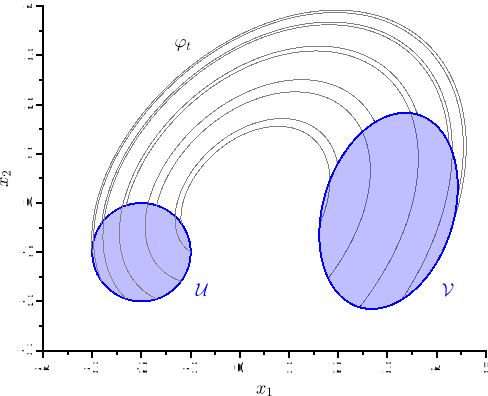
\includegraphics[width=0.75\textwidth]{fluss_diffeom}
\par\end{centering}
\caption{Überführung der Menge~$\mathcal{U}$ in die Menge~$\mathcal{V}$
mit dem Fluss der linearen Differentialgleichung aus Beispiel~\ref{exa:invertierbarkeit-fluss-lin-dgl}\label{fig:Invertierbarkeit-des-Flusses-linear}}
\end{figure}

Mit Prop.~\ref{pro:Lokale-Invertierbarkeit-Fluss} wurde nur die
lokale Invertiertbarkeit des Flusses gezeigt\index{Fluss!Invertierbarkeit}.
Tatsächlich ist der Fluss auf seinem gesamten Existenzbereich invertierbar.
Im Falle eines globalen Flusses ist der bereits verwendete Begriff
der Gruppen\-eigen\-schaft auch im Sinne der Algebra gerechtfertigt:
\begin{remark}
\label{rem:Gruppeneigenschaft}\index{Gruppeneigenschaft}Eine Menge~$\mathcal{G}$
mit einer binären Operation $\circ:\mathcal{G}\times\mathcal{G}\to\mathcal{G}$
heißt \emph{Gruppe}\index{Gruppe}, wenn die Operation~$\circ$ assoziativ
ist, ein neutrales Element besitzt und zu jedem Element der Gruppe
ein inverses Element existiert~\cite{waerden1,bronstein2000,zeidler2003}.
Das Vektorfeld~$f:\mathcal{M}\to\mathbb{R}$ habe den globalen Fluss~$\varphi_{t}$.
Für beliebige $t\in\mathbb{R}$ ist die Abbildung $x\mapsto\varphi_{t}(x)$
ein Diffeomorphismus\index{Diffeomorphismus} auf~$\mathcal{M}$.
Die Menge der Diffeomorphismen ist zusammen mit der durch die Hintereinanderausführung
der Flüsse nach Eigenschaft~(\ref{eq:Gruppeneigenschaft2}) definierten
Operation~$\circ$ eine Gruppe, die man auch als \emph{einparametrige
Transformationsgruppe} bezeichnet~\cite{stephani1994,arnold2001,kuehnel2011}.
\end{remark}
\medskip{}

Zur Untersuchung des nichtlinearen Systems~(\ref{eq:dgl2}) greift
man mitunter auf die Linearisierung entlang einer Trajektorie des
Systems zurück. Dabei wird man auf die Variationsgleichung geführt~\cite[Kap.~{32}]{arnold2001}:
\begin{proposition}
[Variationsgleichung]\label{pro:Variationsgleichung}Sei~$\varphi_{t}$
der Fluss der Dgl.~(\ref{eq:dgl2}) mit einem zweimal stetig differenzierbaren
Vektorfeld $f:\mathcal{M}\to\R^{n}$. Für $p\in\mathcal{M}$ ist
\begin{equation}
X(t):=\varphi_{t}^{\prime}(p)\label{eq:Loesung_Variationsgleichung}
\end{equation}
 die Lösung der matrixwertigen Anfangswertaufgabe 
\begin{equation}
\dot{X}=f^{\prime}(\varphi_{t}(p))\cdot X,\quad X(0)=I.\label{eq:Variationsgleichung}
\end{equation}
\end{proposition}
Gl.~(\ref{eq:Variationsgleichung}) heißt \emph{Variationsgleichung}\index{Variationsgleichung}
von~(\ref{eq:awa2}). Ihre Lösung ist die Ableitung des Flusses der
ursprünglichen Differentialgleichung~(\ref{eq:dgl2}) nach dem Anfangswert.
\begin{svmultproof}
Sei $X$ entsprechend Gl.~(\ref{eq:Loesung_Variationsgleichung})
definiert. Mit Lemma~\ref{lem:Schwarz} gilt 
\[
\begin{array}{ccl}
\dot{X}(t) & = & \frac{\partial}{\partial t}X(t)\\
 & = & \frac{\partial}{\partial t}\frac{\partial}{\partial x}\left.\varphi_{t}(x)\right|_{x=p}\\
 & \stackrel{(\ref{eq:lemma-schwarz})}{=} & \frac{\partial}{\partial x}\frac{\partial}{\partial t}\left.\varphi_{t}(x)\right|_{x=p}\\
 & = & \frac{\partial}{\partial x}\left.\dot{\varphi}_{t}(x)\right|_{x=p}\\
 & = & \frac{\partial}{\partial x}\left.f(\varphi_{t}(x))\right|_{x=p}\\
 & = & \left.f^{\prime}(\varphi_{t}(x))\cdot\varphi_{t}^{\prime}(x)\right|_{x=p}\\
 & = & f^{\prime}(\varphi_{t}(p))\cdot X(t),
\end{array}
\]
d.\,h. $X$ erfüllt die Anfangswertaufgabe~(\ref{eq:Variationsgleichung}).
Satz~\ref{thm:Picard-Lindeloeff} garantiert die Eindeutigkeit der
Lösung. Damit hat jede Lösung von~(\ref{eq:Variationsgleichung})
die Form $X(t)=\varphi_{t}^{\prime}(p)$.
\end{svmultproof}

Die Verwendung einer matrixwertigen Linearisierung mag zunächst verwundern.
Man würde nach der Linearisierung von~(\ref{eq:dgl2}) ein System
der gleichen Dimension erwarten, nämlich ein (lineares) System im
Vektorraum~$\R^{n}$. Der Anfangswert des linearisierten Systems
beschreibt die Anfangsabweichung gegenüber der Referenztrajektorie~$\varphi_{t}(p)$
des zugrundeliegenden nichtlinearen Systems. Als Anfangsabweichungen
kommen beliebige Richtungen im Vektorraum~$\R^{n}$ in Frage, so
dass der Anfangswert der Linearisierung immer als Linearkombinationen
der Basisvektoren $e_{1},\ldots,e_{n}\in\R^{n}$ dargestellt werden
kann. Mit dem matrixwertigen Anfangswert $X(0)=I=(e_{1},\ldots,e_{n})$
betrachtet man simultan die Anfangsabweichungen in Richtung der $n$
Einheitsvektoren (siehe Abb.~\ref{fig:Variationsgleichung_matrixwertig}). 

\begin{figure}
\begin{centering}
\scalebox{0.9}[0.9]{\input{variationsgl_matrix.pdftex_t}}
\par\end{centering}
\caption{Referenztrajektorie $\varphi_{t}(p)$ eines nichtlinearen Systemens
und Trajektorien von Linearisierungen mit Anfangswerten in Richtung
der Einheitsvektoren\label{fig:Variationsgleichung_matrixwertig}}

\end{figure}

Bei verschiedenen Aufgabenstellungen (z.\,B. Empfindlichkeitsuntersuchungen
und Probleme der optimalen Steuerung) benötigt man neben der eigentlichen
Variationsgleichung~(\ref{eq:Variationsgleichung}) auch die \emph{adjungierte
Variationsgleichung}~\cite[Lemma~{4.4.4}]{sontag98}:
\begin{proposition}
[Adjungierte Variationsgleichung]\label{pro:Adjungierte-Variationsgleichung}\index{Variationsgleichung!adjungierte}Sei~$\varphi_{t}$
der Fluss der Dgl.~(\ref{eq:dgl2}) mit einem zweimal stetig differenzierbaren
Vektorfeld $f:\mathcal{M}\to\R^{n}$. Für $p\in\mathcal{M}$ ist 
\begin{equation}
Z(t):=\varphi_{-t}^{\prime}(\varphi_{t}(p))\label{eq:Loesung_Adj_Variationsgl}
\end{equation}
 die Lösung der matrixwertigen Anfangswertaufgabe 
\begin{equation}
\dot{Z}=-Z\cdot f^{\prime}(\varphi_{t}(p)),\quad Z(0)=I.\label{eq:AdjVariationsgleichung}
\end{equation}
\end{proposition}
\begin{svmultproof}
Der Fluss~$\varphi_{t}$ ist ein lokaler Diffeomorphismus. Daher
gilt $\varphi_{-t}(\varphi_{t}(x))=x$ für alle $x$ in der Umgebung
des Anfangswertes~$p$. Differentiation nach~$x$ liefert 
\begin{equation}
\varphi_{-t}^{\prime}(\varphi_{t}(x))\cdot\varphi_{t}^{\prime}(x)=I.\label{eq:Produkt_Variationsgln}
\end{equation}
Eine weitere Differentiation nach~$t$ und das Einsetzen $x=p$ führen
auf 
\[
\frac{\partial}{\partial t}\left(\varphi_{-t}^{\prime}(\varphi_{t}(p))\right)\cdot\varphi_{t}^{\prime}(p)+\varphi_{-t}^{\prime}(\varphi_{t}(p)\cdot\underbrace{\frac{\partial}{\partial t}\left(\varphi_{t}^{\prime}(p)\right)}_{{\displaystyle (*)}}=0.
\]
Der Term~$(*)$ kann durch die rechte Seite der Variationsgleichung~(\ref{eq:Variationsgleichung})
ersetzt werden. Mit $Z(t)$ entsprechend Gl.~(\ref{eq:Loesung_Adj_Variationsgl})
erhält man 
\[
\dot{Z}(t)\cdot\varphi_{t}^{\prime}(p)+Z(t)\cdot f^{\prime}(\varphi_{t}(p))\cdot\varphi_{t}^{\prime}(p)=0.
\]
Multipliziert man diese Gleichung von rechts mit $(\varphi_{t}^{\prime}(p))^{-1}$,
so erhält man die gewünschte Differentialgleichung~(\ref{eq:AdjVariationsgleichung}).
\end{svmultproof}

Die Berechnung der Lösung~(\ref{eq:Loesung_Adj_Variationsgl}) der
adjungierten Variationsgleichung~(\ref{eq:AdjVariationsgleichung})
erscheint auf den ersten Blick aufwendiger als im Fall der Variationsgleichung~(\ref{eq:Variationsgleichung}).
Die im Beweis verwendete Gl.~(\ref{eq:Produkt_Variationsgln}) kann
man in Verbindung mit den Lösungen~(\ref{eq:Loesung_Variationsgleichung})
und~(\ref{eq:Loesung_Adj_Variationsgl}) in der Form 
\begin{equation}
Z(t)\,X(t)=I\label{eq:Produkt-Variationsgleichung}
\end{equation}
angeben. Damit stehen die Zeilen von~$Z(t)$ entlang der Lösung senkrecht
auf den Spalten von~$X(t)$. Dieser Zusammenhang erlaubt die unmittelbare
Berechnung der Lösung~(\ref{eq:Loesung_Adj_Variationsgl}) der adjungierten
Variationsgleichung~(\ref{eq:AdjVariationsgleichung}) mit Hilfe
der Lösung~(\ref{eq:Loesung_Variationsgleichung}): 
\begin{equation}
Z(t)=X^{-1}(t).\label{eq:Loesung_adj_als_Inverse}
\end{equation}


\section*{Übungsaufgaben\addcontentsline{toc}{section}{Übungsaufgaben}}

\begin{aufgabe}Stellen Sie das lineare Vektorfeld 
\[
f(x)=Ax\quad\text{mit}\quad A=\left(\begin{array}{cc}
a_{11} & a_{12}\\
a_{21} & a_{22}
\end{array}\right)
\]
entsprechend Gl.~(\ref{eq:Basisdarstellung-Vektorfelder}) bezüglich
das Basis $\{\tfrac{\partial}{\partial x_{1}},\tfrac{\partial}{\partial x_{2}}\}$
dar.\end{aufgabe}

\begin{aufgabe}\label{aufgabe-gr-Ableitungsregeln}Beweisen Sie die
Aussagen~(\ref{eq:Ableitungsregeln}) von Proposition~\ref{pro:Ableitungsregeln-Felder}.\end{aufgabe}

\begin{aufgabe}Prüfen Sie, ob die Differentialform 
\[
\omega(x)=(2x_{1}-x_{2})x_{3}\,\D x_{1}-x_{1}x_{3}\,\D x_{2}+x_{1}(x_{1}-x_{2})\,\D x_{3}
\]
exakt ist. Berechnen Sie ggf. das zugehörige Potential.\end{aufgabe}

\begin{aufgabe}\label{aufgabe-gr-fluss-roboter}Zu dem Vektorfeld
\[
f(x)=\sin(x_{3})\frac{\partial}{\partial x_{1}}+\cos x_{3}\frac{\partial}{\partial x_{2}}
\]
des mobilen Roboters bestimme man den Fluss $\varphi_{t}$. Geben
Sie dazu einen frei wählbaren Anfangswert $p\in\R^{3}$ vor.\end{aufgabe}

\begin{aufgabe}Zu dem Vektorfeld~$f$ aus Aufgabe~\ref{aufgabe-gr-fluss-roboter}
löse man die matrixwertige Variationsgleichung~(\ref{eq:Variationsgleichung})
sowie die adjungierte Variationsgleichung~(\ref{eq:AdjVariationsgleichung}).\end{aufgabe}

\section*{Lösungen\addcontentsline{toc}{section}{Lösungen}}

\begin{loesung}Die Basisdarstellung lautet
\[
f(x)=\left(a_{11}x_{1}+a_{12}x_{2}\right)\frac{\partial}{\partial x_{1}}+\left(a_{21}x_{1}+a_{22}x_{2}\right)\frac{\partial}{\partial x_{1}}.
\]
\end{loesung}

\begin{loesung}In Gl.~(\ref{eq:Ableitung-SF-VF}) betrachtet man
die Ableitung des mit dem Skalarfeld~$h$ skalierten Vektorfeldes~$f$.
Die Ableitung des $i$-ten Elements nach~$x_{j}$ ergibt sich aus
der Produktregel: 
\[
\frac{\partial\left(h(x)f_{i}(x)\right)}{\partial x_{j}}=\frac{\partial h(x)}{\partial x_{j}}f_{i}(x)+h(x)\frac{\partial f_{i}(x)}{\partial x_{j}}.
\]
 Diese elementweise berechnete Ableitung lässt sich mit 
\[
\frac{\partial\left(h(x)f(x)\right)}{\partial x}=f(x)\,h^{\prime}(x)+h(x)\,f^{\prime}(x)
\]
in Matrix-Notation angeben. Gl.~(\ref{eq:Ableitung-VF-VF}) und~(\ref{eq:Ableitung-Skalarprodukt})
lassen sich in ähnlicher Weise verifizieren.\end{loesung}

\begin{loesung}Die Differentialform ist wegen 
\[
\begin{array}{rcccl}
\frac{\partial\omega_{1}}{\partial x_{2}} & = & -x_{3} & = & \frac{\partial\omega_{2}}{\partial x_{1}}\\
\frac{\partial\omega_{1}}{\partial x_{3}} & = & 2x_{1}-x_{2} & = & \frac{\partial\omega_{3}}{\partial x_{1}}\\
\frac{\partial\omega_{2}}{\partial x_{3}} & = & -x_{1} & = & \frac{\partial\omega_{3}}{\partial x_{2}}
\end{array}
\]
geschlossen. Nach dem Poincaréschen Lemma (Lemma~\ref{lem:poincare})
ist sie dann auch exakt. Das Potential $h(x)=(x_{1}-x_{2})x_{1}x_{3}$
erhält man durch Integration entsprechend Gl.~(\ref{eq:potential-poincare}).\end{loesung}

\begin{loesung}Das Vektorfeld~$f$ kann der nicht\-linearen Differentialgleichung
$\dot{x}=f(x)$ zugeordnet werden. Zusammen mit der Anfangsbedingung
$x(0)=p$ erhält man die Anfangswertaufgabe
\[
\begin{array}{lcllcl}
\dot{x}_{1} & = & \sin x_{3},\quad & x_{1}(0) & = & p_{1},\\
\dot{x}_{2} & = & \cos x_{3},\quad & x_{2}(0) & = & p_{2},\\
\dot{x}_{3} & = & 0,\quad & x_{3}(0) & = & p_{3}.
\end{array}
\]
Die letzte Differentialgleichung hat die konstante Lösung $x_{3}(t)\equiv p_{3}$.
Dadurch haben die ersten zwei Differentialgleichungen eine konstante
rechte Seite und somit die Lösungen 
\begin{eqnarray*}
x_{1}(t) & = & p_{1}+t\sin p_{3},\\
x_{2}(t) & = & p_{2}+t\cos p_{3}.
\end{eqnarray*}
Insgesamt erhält man damit den Fluss 
\begin{equation}
\varphi_{t}(p)=\left(\begin{array}{c}
p_{1}+t\sin p_{3}\\
p_{2}+t\cos p_{3}\\
p_{3}
\end{array}\right).\label{eq:gr-roboter-fluss-f}
\end{equation}
\end{loesung}

\begin{loesung}Die Lösung der matrixwertigen Variationsgleichung~(\ref{eq:Variationsgleichung})
erhält man entsprechend Prop.~\ref{pro:Variationsgleichung} aus
der Ableitung des dem Vektorfeld~$f$ zugehörigen Flusses~(\ref{eq:gr-roboter-fluss-f})
nach dem Anfangswert:
\begin{equation}
X(t)=\varphi_{t}^{\prime}(p)=\left(\begin{array}{ccc}
1 & 0 & \phantom{-}t\cos p_{3}\\
0 & 1 & -t\sin p_{3}\\
0 & 0 & 1
\end{array}\right).\label{eq:loes-gr-Var-X}
\end{equation}
Die Lösung~(\ref{eq:Loesung_Adj_Variationsgl}) der adjungierten
Variationsgleichung~(\ref{eq:AdjVariationsgleichung}) erhält man
entsprechend Gl.~(\ref{eq:Loesung_adj_als_Inverse}) aus der Inversen
von~(\ref{eq:loes-gr-Var-X}):
\[
Z(t)=X^{-1}(t)=\left(\begin{array}{ccc}
1 & 0 & -t\cos p_{3}\\
0 & 1 & \phantom{-}t\sin p_{3}\\
0 & 0 & 1
\end{array}\right).
\]
\end{loesung}

\bibliographystyle{babalpha}
\bibliography{dynamic}

\end{document}
